\documentclass{ieeeaccess}
\usepackage{cite}
\usepackage{amsmath,amssymb,amsfonts}
\usepackage{algorithm}
\usepackage{algpseudocode}
\usepackage{graphicx}
\usepackage{textcomp}
\usepackage{url}
\usepackage{array,tabularx}
\usepackage{booktabs}
\usepackage{bm}

\graphicspath{{figures/}}

\def\BibTeX{{\rm B\kern-.05em{\sc i\kern-.025em b}\kern-.08em
    T\kern-.1667em\lower.7ex\hbox{E}\kern-.125emX}}


\renewcommand{\dbltopfraction}{0.95}
\renewcommand{\dblfloatpagefraction}{0.85}
\setcounter{dbltopnumber}{3}
\renewcommand{\topfraction}{0.95}
\renewcommand{\floatpagefraction}{0.85}
\setcounter{topnumber}{3}
\begin{document}
\history{Date of publication xxxx 00, 0000, date of current version xxxx 00, 0000.}
\doi{}

\title{V-LiDAR: Real-Time Monocular Floor Segmentation and Virtual 2D Scan Synthesis for Autonomous Mobile Robot Obstacle Avoidance}

\author{\uppercase{Hyunwoo Gu}\authorrefmark{1},
\uppercase{Gunmin Yoo}\authorrefmark{1},
\uppercase{Hyunseo Lee}\authorrefmark{1},
\uppercase{Hyun-Mo Kang}\authorrefmark{1},
\uppercase{Min-Seok Lee}\authorrefmark{1},
and \uppercase{Sung Soo Hwang}\authorrefmark{1}, \IEEEmembership{Senior Member, IEEE}}

\address[1]{School of Artificial Intelligence, Computer and Electrical Engineering, Handong Global University, Pohang 37554, Republic of Korea\allowbreak\ (e-mail: 21800030@handong.ac.kr;\allowbreak\ gunminy@handong.ac.kr;\allowbreak\ hslee@handong.ac.kr;\allowbreak\ hmkang012@gmail.com;\allowbreak\ glen@handong.ac.kr;\allowbreak\ sshwang@handong.edu)}

\tfootnote{This research was supported by the ANCHOR program Glocal University 30 through the Gyeongbuk ANCHOR CENTER, funded by the Ministry of Education (MOE) and the Gyeongsangbuk-do, Republic of Korea (2026-ANCHOR-15-119). This work was also supported in part by the National Research Foundation of Korea (NRF) grant funded by the Korean government (MSIT) (No. RS-2025-24683458) and the Handong Global University Academic Research Grant (No. 202500590001). Generative AI tools were utilized solely for English language editing and LaTeX formatting assistance; all research concepts, algorithmic designs, physical experimental validations, and manuscript conclusions were developed entirely by the authors. \textit{Hyunwoo Gu, Gunmin Yoo, Hyunseo Lee, Hyun-Mo Kang, and Min-Seok Lee contributed equally to this work.}}

\markboth
{Gu \headeretal: V-LiDAR: Real-Time Monocular Floor Segmentation and Virtual 2D Scan Synthesis}
{Gu \headeretal: V-LiDAR: Real-Time Monocular Floor Segmentation and Virtual 2D Scan Synthesis}

\corresp{Corresponding author: Sung Soo Hwang (e-mail: sshwang@handong.edu).}

\begin{abstract}
Autonomous mobile robots (AMRs) operating in structured indoor environments predominantly rely on active planar LiDAR sensors for real-time collision avoidance. However, physical LiDAR introduces significant cost, mechanical integration complexity, payload weight, and power draw, while remaining vulnerable to specular reflections on polished floors and beam dropouts through transparent glass. This paper presents \textit{V-LiDAR}, a lightweight, real-time virtual 2D scan synthesis framework that converts monocular RGB images directly into standard ROS~2 \texttt{sensor\_msgs/LaserScan} messages for reactive obstacle avoidance on lightweight mobile robots without dedicated active range sensors. The architecture employs a fine-tuned YOLOv11n-seg model accelerated via Intel OpenVINO FP16, delivering an inference throughput of 78.4\,FPS (12.9\,ms latency) on an onboard Intel Core Ultra 7 155H processor---a 1.7$\times$ speedup over vanilla PyTorch CPU. To eliminate floor glare and occlusion artifacts, we formulate a three-stage post-processing pipeline comprising multi-instance bitwise-OR mask merging, $7 \times 7$ morphological closing, and an asymmetric temporal Exponential Moving Average (EMA, $\alpha=0.6$) bidirectional persistence filter ($N_{\mathrm{onset}}=2, N_{\mathrm{clear}}=2$). Precomputed 2D Euclidean lookup tables map column-wise ground-contact boundary pixels to metric range and angular bins, eliminating runtime trigonometric overhead. In addition, we establish a rigorous mathematical formulation of the near-field optical blind spot ($D_{\min} \approx 2.18$\,m for mounting height $h=1.05$\,m and tilt $\gamma=2.0^\circ$). In comparative benchmarks against foundation depth models, V-LiDAR operates at 78.4\,FPS (12.9\,ms), whereas Depth Anything V2 Small reaches only 1.7\,FPS (601.4\,ms). In 20 consecutive real-world closed-loop obstacle avoidance trials across a 10.0-m trajectory in an open testing hall without pre-built maps, the robot achieved a 90.0\% goal completion rate (18/20 runs) with an average lateral clearance of 1.22\,m, with diagnostic analysis identifying costmap inflation entrapment in the remaining runs.
\end{abstract}

\begin{keywords}
Autonomous mobile robots, obstacle avoidance, monocular vision, virtual LaserScan, floor segmentation, ROS 2 Nav2, optical blind spot, lightweight robotics.
\end{keywords}

\titlepgskip=-21pt

\maketitle

\begin{figure*}[!t]
  \centering
  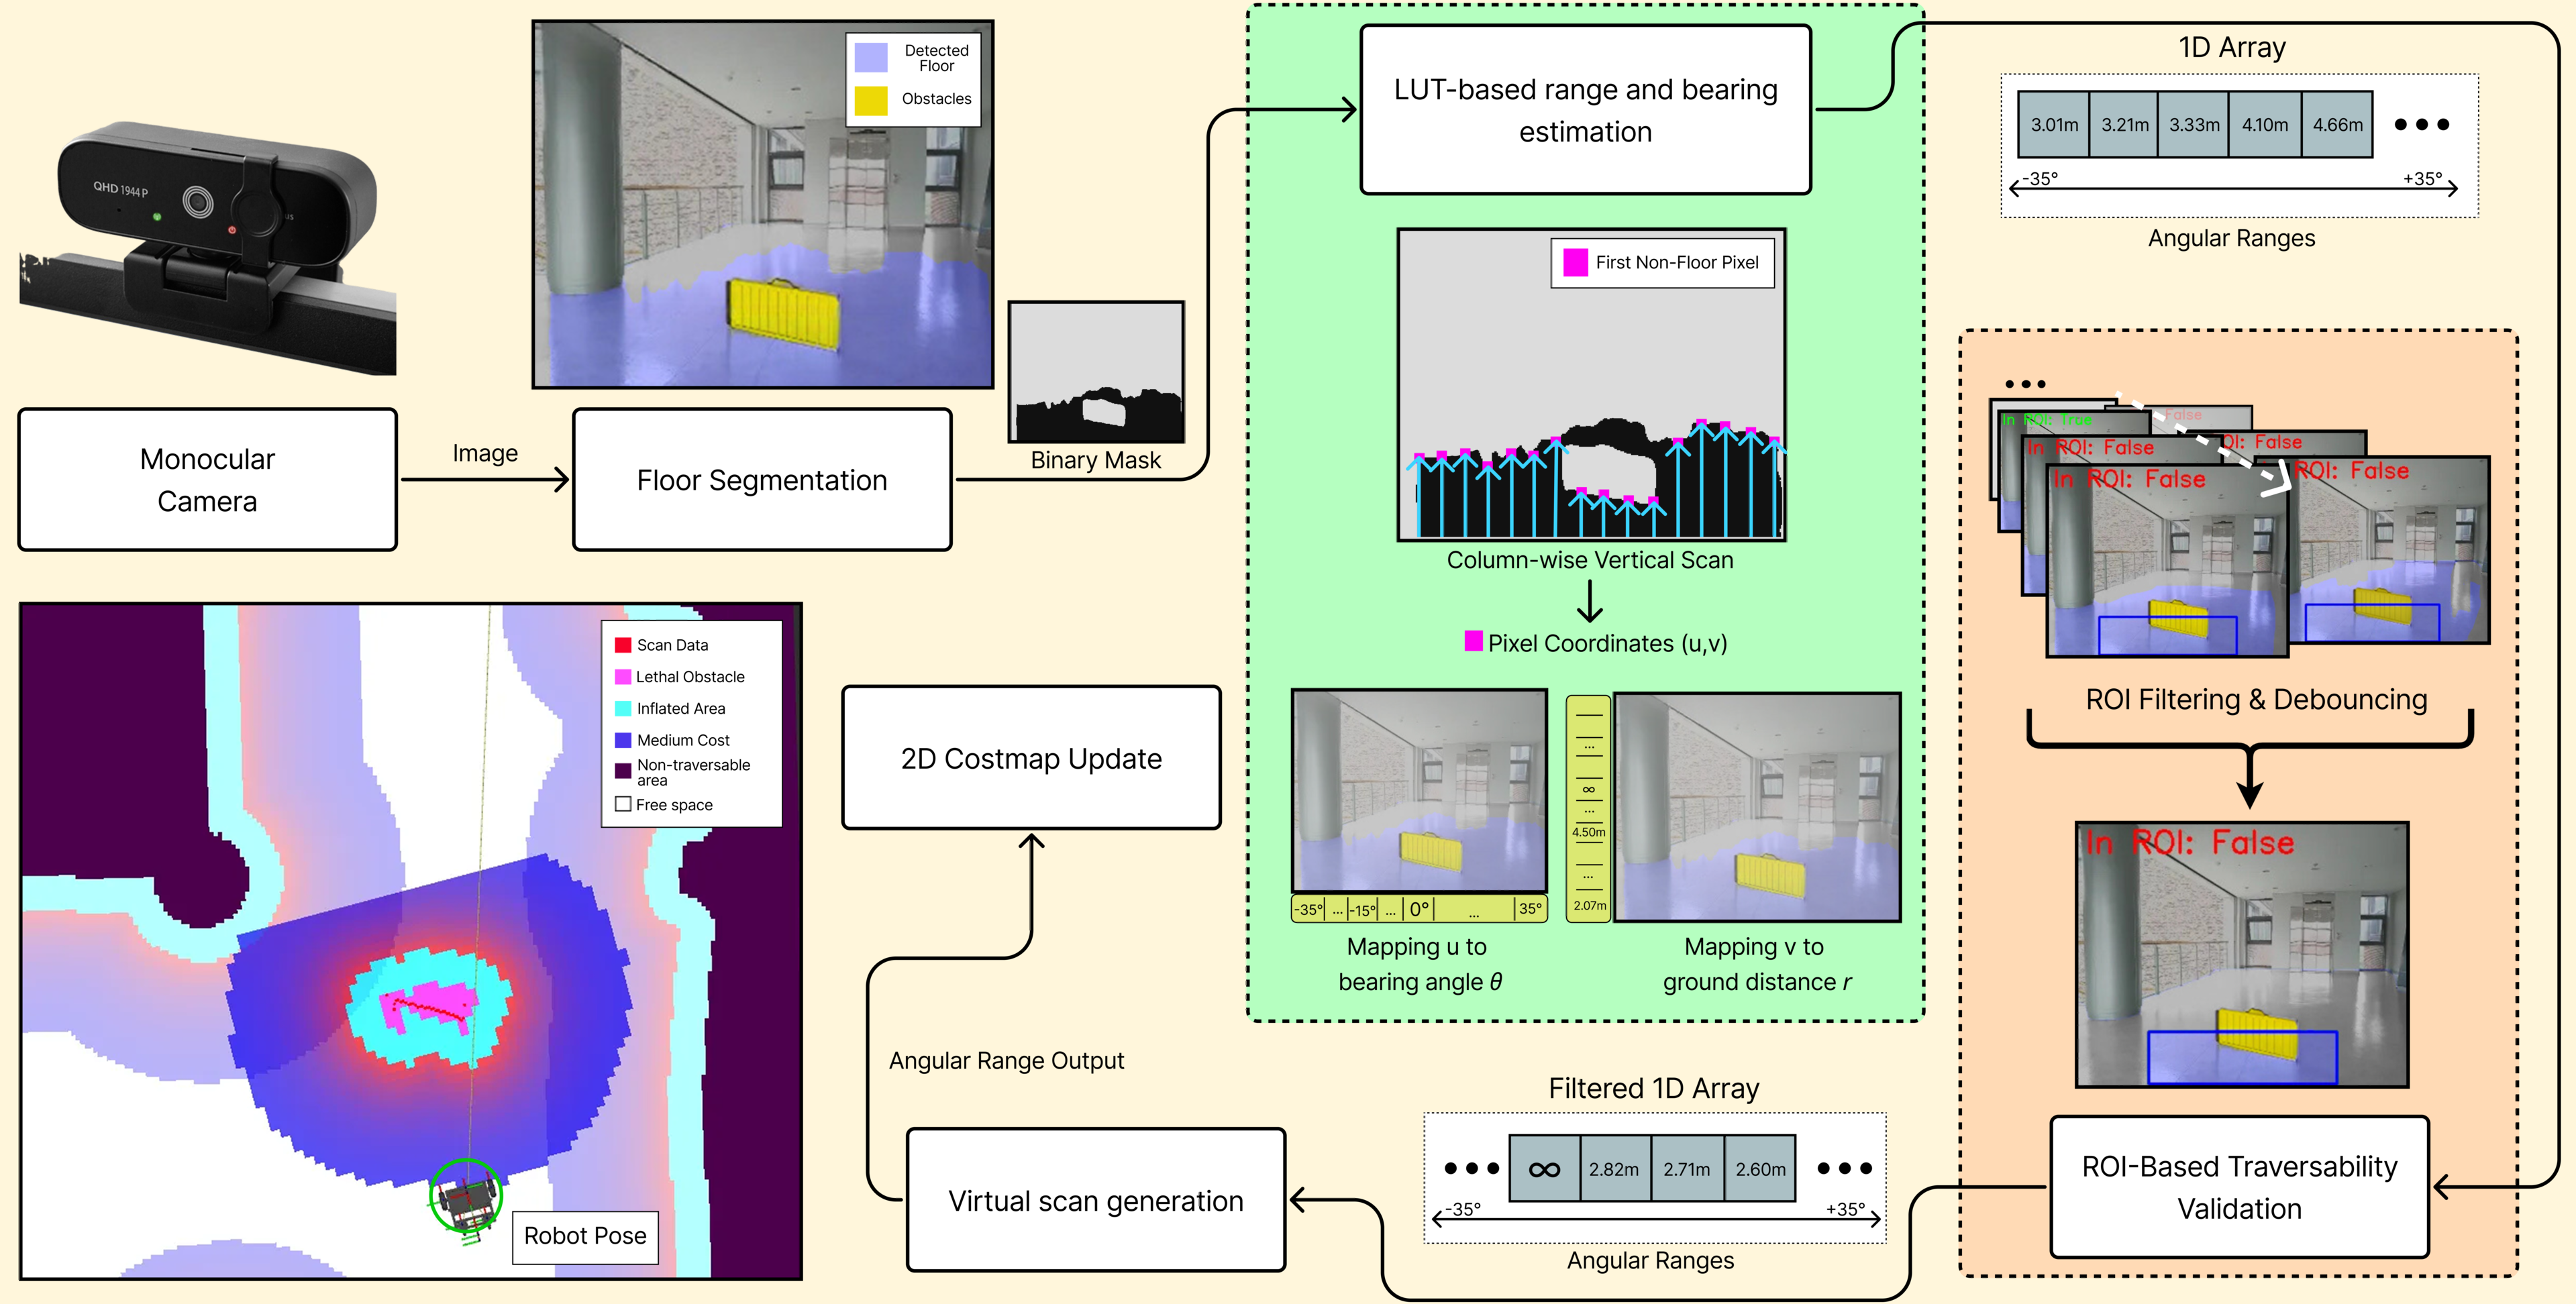
\includegraphics[width=0.93\textwidth]{pipeline}
  \caption{Architectural overview of the proposed vision-based 2D scan generation and obstacle avoidance pipeline. A monocular RGB stream is processed by a fine-tuned YOLOv11n-seg model. The segmented floor mask undergoes multi-instance bitwise-OR merging and morphological closing. Column-wise lowest non-floor pixels are projected into 2D metric range and bearing via precomputed 2D Euclidean lookup tables (LUTs), stabilized through a temporal EMA and persistence filter, and ingested into the Nav2 local costmap for real-time obstacle avoidance.}
  \label{fig:pipeline}
\end{figure*}

\section{Introduction}
\label{sec:introduction}

Autonomous mobile robots (AMRs) are increasingly deployed in diverse structured indoor environments, such as smart warehouses, logistics centers, hospitals, and automated office spaces~\cite{gvrnextgenerationtechnologiesresearchteam_2026_autonomous,liu_2024_a}. Safe and reliable navigation in these shared operational spaces requires robots to continually perceive forward traversable areas, detect dynamic and static obstacles, and generate collision-free trajectories in real time~\cite{macenski_2020_the,yang_2019_semantic}.

Traditionally, indoor AMR navigation frameworks heavily depend on active range sensors, notably two-dimensional planar Light Detection and Ranging (LiDAR) or RGB-D depth sensors~\cite{li_2020_lidar,yusuf_2022_iotbased}. Although LiDAR provides accurate metric measurements with wide fields of view, its integration increases total bill-of-materials (BOM), structural payload, and power draw~\cite{liu_2024_a,alatise2020review}. Furthermore, optical range sensors are inherently prone to measurement dropouts and false occupancy artifacts when encountering specular surfaces, mirrors, polished epoxy floors, and transparent glass partitions~\cite{deepthadamodaran_2023_experimental,yang_2011_on,tibebu_2021_lidarbased,sajjan_2020_clear,singh_2019_multidata}.

In contrast, monocular RGB cameras represent a compact, low-cost, and ubiquitous alternative for lightweight robotic platforms~\cite{kim2022opensource}. Recent advancements in deep neural networks have made it feasible to extract dense geometric depth or semantic floor masks directly from monocular RGB video streams at high frame rates~\cite{shariqfarooqbhat_2021_adabins,ranftl_2021_vision,ultralytics_2024_ultralytics}. However, visual outputs generated by deep learning models (such as pixel-level semantic segmentation masks or relative depth maps) are not formatted as planar range measurements. Mature, production-grade robotic navigation architectures---most prominently the Robot Operating System 2 (ROS 2) and Nav2 navigation stack~\cite{macenski_2022_robot,macenski_2023_from}---expect metric spatial observations packaged as standard \texttt{sensor\_msgs/LaserScan} or \texttt{sensor\_msgs/PointCloud2} messages~\cite{openrobotics_sensor_msgslaserscan}. Consequently, a significant architectural interface gap remains between monocular visual segmentation and standard 2D local costmap planners~\cite{openrobotics_2020_depthimage_to_laserscan,opennavigationllc_2023_costmap}.

This paper proposes an integrated, real-time virtual 2D scan generation pipeline that converts monocular floor-segmentation outputs into standard ROS 2 \texttt{LaserScan} messages as a cost-effective, lightweight perception alternative for mobile robot obstacle avoidance without physical LiDAR sensors. The system leverages an efficient Ultralytics YOLOv11n-seg model to infer binary traversable ground masks~\cite{ultralytics_2024_ultralytics}. Instead of relying on computationally heavy per-frame 3D back-projection, two precomputed 2D Euclidean lookup tables (LUTs) map image pixel coordinates directly to metric range and angular scan bins based on calibrated camera intrinsics and extrinsics.

A critical challenge encountered in vision-based ground detection is vulnerability to illumination variance, glossy floor glare, and mask fragmentation when an obstacle occludes part of the floor. To overcome these failure modes, we introduce a robust three-stage stabilization framework: (i) multi-instance mask bitwise-OR merging, (ii) morphological closing with a rectangular kernel to eliminate reflection-induced holes, and (iii) a dual-speed temporal Exponential Moving Average (EMA) and persistence counter to eliminate scan jitter while retaining immediate response to newly appearing obstacles. Furthermore, we provide a formal trigonometric derivation of the near-field optical blind spot ($D_{\min} \approx 2.18$\,m) dictated by camera mounting height and pitch angle, establishing why ground-contact segmentation cannot resolve obstacles closer than this physical boundary.

The primary contributions of this paper are summarized as follows:
\begin{enumerate}
  \item \textbf{Real-Time Virtual Scan Architecture (V-LiDAR)}: We design an end-to-end perception pipeline that converts monocular floor segmentation masks into standard ROS 2 \texttt{LaserScan} observations via calibrated 2D Euclidean lookup tables, bridging the interface gap between monocular vision and the Nav2 local costmap without online trigonometric latency.
  \item \textbf{Edge AI Acceleration and MDE Comparative Benchmark}: We implement OpenVINO FP16 optimizations achieving 78.4\,FPS (12.9\,ms latency) on an onboard Intel Core Ultra 7 155H CPU. Benchmarks across 200 synchronized frames against MDE baselines (MiDaS v2.1 and Depth Anything V2) show that while dense depth fails to meet 10\,Hz control deadlines (1.7\,FPS, 601.4\,ms), V-LiDAR provides a $7.7\times$ real-time timing margin with only 2.84\,M parameters.
  \item \textbf{Three-Stage Reflection and Flicker Suppression Pipeline}: We introduce a stabilization framework coupling multi-instance bitwise-OR mask fusion, $7 \times 7$ morphological closing, and an asymmetric dual-speed temporal EMA and bidirectional persistence filter ($N_{\mathrm{onset}}=2, N_{\mathrm{clear}}=2$). In a systematic component ablation study, this pipeline suppresses specular floor reflection noise from 38.5\% down to 1.8\% and reduces distance jitter ($\sigma$) by 97.9\%.
  \item \textbf{Mathematical Formulation of the Near-Field Optical Blind Spot}: We formally derive the near-field optical blind spot ($D_{\min} = 2.178$\,m for $h = 1.05$\,m, $\gamma = 2.0^\circ$), theoretically demonstrating that ground-contact cropping is a geometric consequence of mounting optics and ground-plane geometry. We also derive sensitivity derivatives and analyze costmap inflation entrapment in narrow corridors ($<2.2$\,m).
  \item \textbf{Extensive Real-World Navigation Validation}: We validate the pipeline through static ranging and 20 consecutive 10.0-meter autonomous obstacle avoidance trials on an OMO-R1 mobile robot without a static map. The system attains a promising 90.0\% goal completion rate (18/20 runs) under static single-obstacle test scenarios, accompanied by a root-cause analysis of local planner costmap interactions.
\end{enumerate}

The remainder of this paper is structured as follows. Section~\ref{sec:related_work} reviews related literature. Section~\ref{sec:proposed_method} details the proposed methodology. Section~\ref{sec:blind_spot} mathematically analyzes the optical blind spot. Section~\ref{sec:experiments} presents static and closed-loop navigation experiments. Section~\ref{sec:discussion} discusses failure cases and operational boundaries, and Section~\ref{sec:conclusion} concludes the paper.

\section{Related Work and Technical Challenges}
\label{sec:related_work}

\subsection{Active Range Sensing and Its Limitations}
Planar 2D LiDAR and 3D time-of-flight (ToF) sensors serve as standard modalities for occupancy grid mapping, SLAM, and collision avoidance~\cite{li_2020_lidar,thrun_2010_probabilistic,elfes_1989_using}. Despite high precision, optical sensors face documented vulnerabilities: polished marble, specular waxed vinyl tiles, and wet surfaces induce total internal reflection, deflecting laser beams and creating false free-space holes~\cite{deepthadamodaran_2023_experimental,yang_2011_on,zhang2023robust}. Additionally, glass doors and transparent barriers produce missing returns or distorted obstacle boundaries~\cite{tibebu_2021_lidarbased,wang_2017_detecting}. These physical constraints, alongside payload and power limits on low-cost AMRs, motivate alternative sensing and multi-sensor fusion paradigms~\cite{alatise2020review}.

\subsection{Monocular Depth Estimation vs. Semantic Floor Segmentation}
\label{subsec:mde_vs_floor}
Monocular depth estimation (MDE) aims to infer per-pixel distance from single RGB images. Transformer-based architectures such as AdaBins~\cite{shariqfarooqbhat_2021_adabins} and DPT~\cite{ranftl_2021_vision} utilize adaptive binning, while recent foundation models such as MiDaS~\cite{ranftl_2020_towards} and Depth Anything V1/V2~\cite{yang_2024_depth} demonstrate strong zero-shot generalization.

Despite their visual quality, deploying general-purpose MDE models on mobile robots faces two fundamental impediments:
\begin{enumerate}
  \item \textbf{Metric Scale Ambiguity}: Foundation depth models output scale- and shift-invariant relative disparity rather than metric depth. Converting relative disparity to metric meters requires ground-plane calibration or auxiliary sensors, which are vulnerable to drift.
  \item \textbf{Prohibitive Computational Latency}: Vision Transformer (ViT) backbones contain $24\text{--}335$\,M parameters. As benchmarked in Section~\ref{subsec:baseline_benchmark}, Depth Anything V2 Small requires $601.4$\,ms per frame on edge CPU (1.7\,FPS), breaching Nav2's 10\,Hz control deadline by a factor of 6.0.
\end{enumerate}

To bypass metric ambiguity and computational bottlenecks, semantic floor segmentation isolates traversable ground directly as a classification task for mobile robots~\cite{sevastopoulos2022survey,hyun2022street}. Ultralytics YOLOv11n-seg~\cite{ultralytics_2024_ultralytics} and real-time networks such as BiSeNet~V2~\cite{yu2021bisenetv2} identify navigable ground boundaries at high frame rates~\cite{wang2023realtime}. With an ultra-compact backbone ($2.84$\,M parameters), YOLOv11n-seg compiles into an OpenVINO FP16 runtime delivering sub-$15$\,ms latency. Projecting the lowest non-floor pixel boundaries onto the ground plane derives metric distance deterministically via Euclidean geometry, eliminating scale ambiguity while achieving $>75$\,FPS throughput.

\subsection{Comprehensive Sensory Modality Comparison}
\label{subsec:sensory_comparison}

To contextualize the practical and economic value of V-LiDAR within indoor mobile robotics, Table~\ref{tab:sensory_comparison} compares the proposed framework against conventional 2D LiDAR, 3D solid-state LiDAR, RGB-D depth sensors, and monocular dense MDE across seven operational dimensions.

\begin{table*}[!t]
  \centering
  \footnotesize
  \caption{Comprehensive Comparison Across Robotic Obstacle Avoidance Sensory Modalities}
  \label{tab:sensory_comparison}
  \begin{tabularx}{\textwidth}{@{}p{2.2cm}p{2.4cm}cccccX@{}}
    \toprule
    Modality & Representative Hardware & Cost (USD) & Weight & Power & Horiz. FOV & Metric Scale? & Primary Vulnerability / Compute Overhead \\
    \midrule
    \textbf{2D Planar LiDAR} & RPLIDAR A2 / UST-10LX & \$300--\$1,800 & 190--400\,g & 4.0--8.0\,W & 270$^\circ$--360$^\circ$ & Direct (ToF) & Glass penetration; waxed floor beam deflections; mechanical motor wear. \\
    \textbf{3D Solid-State LiDAR} & Livox Mid-360 / Ouster & \$800--\$4,000 & 265--450\,g & 6.5--15.0\,W & 360$^\circ \times 59^\circ$ & Direct (ToF) & High hardware cost; heavy 3D pointcloud downsampling compute on edge CPU. \\
    \textbf{RGB-D Camera} & Intel RealSense D435i & \$350--\$500 & 72\,g & 2.5--3.5\,W & 86$^\circ \times 57^\circ$ & Direct (Stereo/IR) & Extreme sunlight / glossy floor IR scattering; limited outdoor range. \\
    \textbf{Monocular Dense MDE} & Standard RGB + DepthAnyV2 & $<$ \$20 & $<$ 30\,g & $<$ 1.0\,W & 70$^\circ$--90$^\circ$ & Relative only & Uncalibrated scale; prohibitive transformer latency ($>600$\,ms / 1.7\,FPS). \\
    \textbf{V-LiDAR (Proposed)} & \textbf{Standard RGB + OpenVINO} & $<$ \textbf{\$20} & $<$ \textbf{30\,g} & $<$ \textbf{1.0\,W} & \textbf{70.0$^\circ$ (141 ch.)} & \textbf{Direct (2D LUT)} & \textbf{Near-field blind spot ($<2.18$\,m); lightweight compute (12.9\,ms).} \\
    \bottomrule
  \end{tabularx}
\end{table*}

Table~\ref{tab:sensory_comparison} highlights that physical 2D and 3D LiDAR sensors incur hardware costs ranging from \$300 to \$4,000 and draw 4.0--15.0\,W of electrical power. While LiDAR provides omnidirectional coverage, it remains susceptible to specular deflection on waxed floors and transparent glass doors. In contrast, V-LiDAR leverages a commodity camera ($<\$20$, $<30$\,g, $<1$\,W) and eliminates the metric scale ambiguity of general MDE models through precomputed 2D lookup tables, presenting a low-cost, energy-efficient complementary perception alternative for service robots operating in structured indoor environments.

\subsection{Perception-to-Navigation Middleware Interface}
Modern mobile robots rely on ROS 2 for process orchestration~\cite{quigley_2009_ros,macenski_2022_robot,wei2025ros}, with the Nav2 stack standardizing planning and obstacle representation~\cite{macenski_2020_the,macenski_2023_from,hu2025improved}. Nav2 maintains layered 2D costmaps~\cite{opennavigationllc_2023_costmap} consuming \texttt{sensor\_msgs/LaserScan} streams~\cite{openrobotics_sensor_msgslaserscan}. Conversion utilities such as \texttt{depthimage\allowbreak\_to\allowbreak\_laserscan}~\cite{openrobotics_2020_depthimage_to_laserscan} and \texttt{pointcloud\allowbreak\_to\allowbreak\_laserscan}~\cite{openrobotics_2015_pointcloud_to_laserscan} require calibrated depth images or point clouds, which monocular cameras cannot directly provide.

Bridging this gap requires generating synthetic 2D scans from monocular images under flat-ground assumptions~\cite{moravec_1985_high,fox_1997_the}. However, frame jitter or latency induces path oscillations or false stops in Nav2 local planners~\cite{fox_1997_the,kobayashi2022local,opennavigationllc_2025_denoise}. Ensuring temporal stability and spatial consistency is thus essential. This framework deliberately targets local reactive costmaps for collision avoidance; global visual SLAM, 3D reconstruction, and loop closure are decoupled and left to higher-level modules.

\section{Proposed Method}
\label{sec:proposed_method}

Table~\ref{tab:notation} summarizes the mathematical notations used throughout this section.

\begin{table}[t]
  \centering
  \caption{Mathematical Notation Used in the Proposed Pipeline}
  \label{tab:notation}
  \begin{tabularx}{\linewidth}{@{}p{0.32\linewidth}X@{}}
    \toprule
    Symbol & Description \\
    \midrule
    $W, H$ & Image width and height in pixels ($320 \times 256$) \\
    $f_x, f_y$ & Camera focal lengths along horizontal/vertical axes \\
    $(c_x, c_y)$ & Principal point coordinates in image plane \\
    $h, \gamma$ & Camera height above ground ($1.05$\,m) and pitch angle ($2.0^\circ$) \\
    $u, v$ & Pixel column and row indices ($0 \le u < W, 0 \le v < H$) \\
    $N_{\mathrm{ang}}$ & Number of virtual angular scan bins ($N_{\mathrm{ang}} = 141$) \\
    $L_{\mathrm{bin}}[u]$ & Column-to-angular-bin lookup table \\
    $L_{\mathrm{range}}[v, u]$ & 2D Euclidean distance lookup table \\
    $M_{\mathrm{seg}}[v, u]$ & Binary floor segmentation mask ($1=\text{floor}, 0=\text{obstacle}$) \\
    $S[i]$ & Virtual scan distance in angular channel $i$ \\
    $\alpha$ & Temporal EMA smoothing factor ($\alpha = 0.6$) \\
    $N_{\mathrm{onset}}, N_{\mathrm{clear}}$ & Bidirectional persistence frame counts ($N_{\mathrm{onset}}=2, N_{\mathrm{clear}}=2$) \\
    $c_{\mathrm{conf}}$ & Floor segmentation confidence threshold ($c_{\mathrm{conf}} = 0.15$) \\
    \bottomrule
  \end{tabularx}
\end{table}

\subsection{System Architecture Overview}
The overall pipeline is depicted in Fig.~\ref{fig:pipeline}. The forward-facing RGB camera publishes uncompressed video frames at 30\,Hz. A ROS 2 node synchronizes image reception, resizes incoming frames to a standardized resolution ($W=320, H=256$), and invokes the YOLOv11n-seg model at a fixed inference rate of 10\,Hz. The generated binary mask undergoes multi-instance bitwise-OR combination and morphological closing. For each image column within the valid field of view, the lowest non-floor pixel is identified as the ground-contact point. Precomputed 2D lookup tables translate pixel coordinates into radial distances and angular bins. The raw channel distances are filtered using a temporal EMA and persistence algorithm and published to the ROS 2 topic \texttt{/scan} as a standard \texttt{sensor\_msgs/LaserScan} message.

\subsection{Floor Segmentation and Multi-Instance Mask Merging}
\label{subsec:floor_seg}
Traversable floor regions are distinguished using the lightweight YOLOv11n-seg model~\cite{ultralytics_2024_ultralytics}, fine-tuned on custom indoor facility datasets under varying illumination. The network outputs a set of $K$ instance segmentation masks $\{m_k\}_{k=1}^K$ using confidence threshold $c_{\mathrm{conf}} = 0.15$, where each $m_k \in \{0, 1\}^{H \times W}$.

In real-world navigation, obstacles resting on the ground frequently split the continuous floor into multiple disconnected visual components (e.g., left floor patch, right floor patch, and distant background floor). A conventional segmentation inference pipeline that selects only the highest-confidence single mask ($m_0$) discards up to 80\% of the valid traversable area, creating a false visual barrier. To eliminate this issue, our system merges all detected floor masks via an element-wise bitwise-OR reduction:
\begin{equation}
  M_{\mathrm{raw}}[v, u] = \bigvee_{k=1}^K m_k[v, u], \quad \forall (v, u) \in [0, H-1] \times [0, W-1].
\end{equation}
If no floor instances are detected (e.g., when the camera lens is physically occluded), $M_{\mathrm{raw}}$ defaults to an all-zero matrix.

\subsection{Morphological Artifact Suppression}
Specular reflection from polished epoxy or linoleum surfaces frequently creates dark, non-floor holes inside genuine traversable regions. To fill these spurious inner holes and smooth irregular boundary noise, a morphological closing operation (dilation followed by erosion) is applied using a structuring element $B$:
\begin{equation}
  M_{\mathrm{seg}} = (M_{\mathrm{raw}} \oplus B) \ominus B,
\end{equation}
where $B$ is configured as a $7 \times 7$ rectangular structuring kernel applied with two iterations:
\begin{equation}
  B = \mathbf{1}_{7 \times 7}.
\end{equation}
This operation effectively bridges reflection-induced gaps of up to 6 pixels caused by overhead lighting without corrupting genuine obstacle boundaries.

\subsection{2D Euclidean Range and Bearing Estimation}
\label{subsec:lut}
To achieve real-time conversion without online trigonometric operations, we precompute two static lookup tables: a Column-to-Bin LUT ($L_{\mathrm{bin}}$) and a 2D Euclidean Distance LUT ($L_{\mathrm{range}}$).
Under a pinhole camera model, an image coordinate $(u, v)$ corresponds to ray angles in camera optical coordinates:
\begin{align}
  \theta(u) &= \arctan\left(\frac{u - c_x}{f_x}\right), \\
  \phi(v)   &= \arctan\left(\frac{v - c_y}{f_y}\right),
\end{align}
where $\theta(u)$ is the horizontal azimuth and $\phi(v)$ is the vertical optical elevation angle. With the camera mounted at physical height $h$ and tilted downward by pitch angle $\gamma$, the net downward depression angle is $\alpha(v) = \phi(v) + \gamma$.

For any ray intersecting a locally flat ground plane, the forward longitudinal distance $X(v)$ and lateral distance $Y(u, v)$ from the camera origin are:
\begin{align}
  X(v) &= \frac{h}{\tan(\phi(v) + \gamma)}, \quad (\phi(v) + \gamma > 0), \\
  Y(u, v) &= X(v) \cdot \tan(\theta(u)).
\end{align}
Conventional 1D lookup tables assume that radial distance depends strictly on row index $v$, ignoring lateral ray expansion towards image edges. To avoid radial distortion at large azimuth angles, our system constructs a true 2D Euclidean distance LUT:
\begin{equation}
  L_{\mathrm{range}}[v, u] = \sqrt{X(v)^2 + Y(u, v)^2} = \frac{h \cdot \sec(\theta(u))}{\tan(\phi(v) + \gamma)}.
\end{equation}
The horizontal bearing is mapped into one of $N_{\mathrm{ang}}$ discrete angular scan bins covering $[-35.0^\circ, +35.0^\circ]$ at $0.5^\circ$ increments:
\begin{equation}
  L_{\mathrm{bin}}[u] = \operatorname{round}\left(\frac{\theta(u) - \theta_{\min}}{\Delta \theta}\right),
\end{equation}
where $\Delta \theta = 0.5^\circ \times (\pi / 180)$ and $N_{\mathrm{ang}} = 141$.

\subsection{Virtual Scan Generation Algorithm}
The column-wise scan extraction procedure is formalized in Algorithm~\ref{alg:virtual_scan}. The scan array $S$ is initialized to infinity. To avoid false readings from ceiling lights and distant horizon boundaries, scanning is restricted to rows below the horizon threshold $y_{\min} = 120$ ($v \in [y_{\min}, H-1]$). For each column $u$, the lowest non-floor pixel $v^*$ corresponds to the ground-obstacle contact line. Because digital image row index $v$ increases downwards ($v=0$ at top, $v=H-1$ at bottom), the maximum index $v^* = \max(\mathcal{V}_u)$ physically identifies the lowest ground-contact point.

\begin{algorithm}[t]
\caption{Virtual LaserScan Generation}
\label{alg:virtual_scan}
\begin{algorithmic}[1]
\Require Segmentation mask $M_{\mathrm{seg}}$, LUTs $L_{\mathrm{range}}$ and $L_{\mathrm{bin}}$, horizon cutoff $y_{\min}$, scan bins $N_{\mathrm{ang}}$
\Ensure Filtered virtual scan array $S[1 \dots N_{\mathrm{ang}}]$
\State Initialize raw distance array $D_{\mathrm{raw}}[i] \gets \infty$ for all $i \in [1, N_{\mathrm{ang}}]$
\For{each image column $u \in [0, W-1]$}
    \State $\mathcal{V}_u \gets \{v \mid y_{\min} \le v < H \text{ and } M_{\mathrm{seg}}[v, u] = 0\}$
    \If{$\mathcal{V}_u \ne \emptyset$}
        \State $v^* \gets \max(\mathcal{V}_u)$ \Comment{Lowest non-floor pixel}
        \State $i \gets L_{\mathrm{bin}}[u]$
        \State $d \gets L_{\mathrm{range}}[v^*, u]$
        \State $D_{\mathrm{raw}}[i] \gets \min(D_{\mathrm{raw}}[i], d)$
    \EndIf
\EndFor
\State $S \gets \textsc{ApplyTemporalFilter}(D_{\mathrm{raw}})$
\State \Return $S$
\end{algorithmic}
\end{algorithm}

\subsection{Temporal EMA and Bidirectional Persistence Filtering}
\label{subsec:temporal_filter}
Raw frame-by-frame distance measurements $D_{\mathrm{raw}}[i]$ are susceptible to segmentation boundary flickering. Directly ingesting fluctuating distance estimates into local costmaps induces dynamic cost oscillation. We formulate an asymmetric dual-state temporal filter with bidirectional persistence that handles obstacle onset and clearance differently:

\begin{enumerate}
  \item \textbf{Persistence-Gated Obstacle Onset}: When an obstacle appears in a channel previously considered free ($D_{\mathrm{raw}}[i] < \infty$ and $S_{\mathrm{prev}}[i] = \infty$), an onset counter increments ($C_{\mathrm{obs}}[i] \gets C_{\mathrm{obs}}[i] + 1$). The obstacle is registered ($S[i] = D_{\mathrm{raw}}[i]$) only after persisting for $N_{\mathrm{onset}} = 2$ consecutive frames, filtering out transient single-frame specular glare spikes.
  \item \textbf{Continuous Obstacle Tracking}: When an obstacle persists across successive frames, an Exponential Moving Average (EMA) with smoothing coefficient $\alpha = 0.6$ is applied:
  \begin{equation}
    S[i] = \alpha \cdot D_{\mathrm{raw}}[i] + (1 - \alpha) \cdot S_{\mathrm{prev}}[i], \quad C_{\mathrm{inf}}[i] = 0.
  \end{equation}
  \item \textbf{Persistence-Gated Obstacle Clearing}: When a channel transitions from occupied to clear ($D_{\mathrm{raw}}[i] = \infty$ and $S_{\mathrm{prev}}[i] < \infty$), an idle counter $C_{\mathrm{inf}}[i]$ increments:
  \begin{equation}
    C_{\mathrm{inf}}[i] \gets C_{\mathrm{inf}}[i] + 1.
  \end{equation}
  The distance is cleared to infinity only after the clear state persists for $N_{\mathrm{clear}} = 2$ consecutive frames:
  \begin{equation}
    S[i] = \begin{cases} \infty, & \text{if } C_{\mathrm{inf}}[i] \ge N_{\mathrm{clear}}, \\ S_{\mathrm{prev}}[i], & \text{otherwise.} \end{cases}
  \end{equation}
\end{enumerate}
This bidirectional persistence provides robust collision response while eliminating both single-frame phantom obstacles and false-clear flickers caused by transient glare.

\subsection{Edge AI Optimization and Runtime Acceleration}
\label{subsec:edge_acceleration}
To guarantee deterministic execution on embedded AMR computing platforms lacking dedicated discrete GPUs, the YOLOv11n-seg network was compiled into an optimized Intel OpenVINO FP16 Intermediate Representation (IR). The optimization process applies layer fusion, constant folding, and half-precision floating-point (FP16) precision conversion and graph optimization, reducing the model footprint from 5.8\,MB to 5.4\,MB without loss of segmentation fidelity.

During online navigation, the ROS 2 node maintains an asynchronous inference queue (\texttt{AsyncInferQueue}) with two parallel infer requests. Incoming camera frames ($640 \times 480$ at 30\,FPS) are ingested into shared memory, bilinearly downsampled to $320 \times 256$, and dispatched to the OpenVINO engine executing across the Performance cores (P-cores) of the Intel Core Ultra 7 155H processor. As quantified in Section~\ref{subsec:baseline_benchmark}, this edge acceleration achieves an average inference latency of $12.9 \pm 1.9$\,ms (78.4\,FPS), comfortably exceeding the camera acquisition rate and freeing CPU bandwidth for simultaneous Nav2 trajectory planning.

\subsection{Three-Sector Angular Channel Partitioning}
\label{subsec:sector_partitioning}
The generated virtual scan consists of $N_{\mathrm{ang}} = 141$ discrete angular channels spanning a symmetric horizontal field of view of $\theta \in [-35.0^\circ, +35.0^\circ]$ at $\Delta \theta = 0.5^\circ$ angular increments. To interface effectively with Nav2's local trajectory critics, the scan channels are partitioned into three functional spatial sectors:
\begin{align}
  \mathcal{S}_{\mathrm{left}}   &= \{i \mid 0 \le i \le 46\},   \quad \theta \in [-35.0^\circ, -12.0^\circ), \\
  \mathcal{S}_{\mathrm{center}} &= \{i \mid 47 \le i \le 93\},  \quad \theta \in [-11.5^\circ, +11.5^\circ], \\
  \mathcal{S}_{\mathrm{right}}  &= \{i \mid 94 \le i \le 140\}, \quad \theta \in (+12.0^\circ, +35.0^\circ].
\end{align}
The central sector $\mathcal{S}_{\mathrm{center}}$ covers the direct $23.0^\circ$ frontal collision corridor, precisely matching the lateral clearance required by the robot's circular footprint ($r_{\mathrm{robot}} = 0.33$\,m) at distances between $2.2$\,m and $5.0$\,m. The lateral sectors $\mathcal{S}_{\mathrm{left}}$ and $\mathcal{S}_{\mathrm{right}}$ monitor flanking wall clearance and guide the DWB controller's \texttt{BaseObstacle} and \texttt{PathAlign} trajectory scoring during evasive maneuvers.

\subsection{End-to-End Latency Budget}
\label{subsec:latency_budget}
The end-to-end computational pipeline operates within a rigorous timing budget. On the physical OMO-R1 platform, per-frame execution decomposes into:
\begin{itemize}
  \item Camera frame acquisition and shared-memory transfer: $3.2 \pm 0.4$\,ms,
  \item Frame downsampling ($640\times480 \rightarrow 320\times256$) and normalization: $1.1 \pm 0.2$\,ms,
  \item OpenVINO FP16 floor segmentation inference: $12.9 \pm 1.9$\,ms,
  \item Multi-instance mask merging and $7\times7$ morphological closing (two iterations): $2.4 \pm 0.3$\,ms,
  \item 2D Euclidean LUT column scan extraction: $1.2 \pm 0.1$\,ms,
  \item Asymmetric temporal EMA and persistence filtering: $0.3 \pm 0.05$\,ms,
  \item ROS 2 \texttt{LaserScan} message serialization and TF broadcast: $0.4 \pm 0.1$\,ms.
\end{itemize}
The cumulative latency is $T_{\mathrm{total}} = 21.5 \pm 2.4$\,ms ($\sim 46.5$\,Hz effective throughput). Because Nav2's local costmap updates at 10\,Hz ($100$\,ms period), our virtual scan pipeline consumes less than 22\% of each control epoch, providing sufficiently low latency to comfortably satisfy the standard 10\,Hz Nav2 control epoch without sensory queuing.

\subsection{ROS 2 Nav2 Costmap Integration}
The filtered scan array $S$ is formatted into a standard \texttt{sensor\_msgs/LaserScan} message with frame identifier \texttt{lidar\_link}. Static coordinate frames are linked via a TF broadcaster defining the forward-facing camera sensor mast mounted 0.55\,m behind the wheel axle center on the OMO-R1 chassis:
\begin{equation}
  \mathbf{T}_{\mathrm{base\_link}}^{\mathrm{lidar\_link}} = [-0.55\,\text{m}, 0.0\,\text{m}, 0.0\,\text{m}]^T.
\end{equation}
Nav2's local costmap incorporates a 2D obstacle layer (\texttt{ObstacleLayer}) subscribing to \texttt{/scan}, with raytracing enabled up to 6.0\,m and marking up to 5.0\,m. To accommodate the virtual scan's forward-limited field of view, the global path planner employs \texttt{nav2\_navfn\_planner}\allowbreak\texttt{/NavfnPlanner} with $A^*$ heuristics for continuous replanning around newly perceived obstacle costs.

\section{Theoretical Analysis of Near-Field Optical Blind Spot}
\label{sec:blind_spot}

Distance estimation relying on ground segmentation inherently exhibits a near-field optical blind spot. In this section, we mathematically derive the minimum observable ground distance ($D_{\min}$) and examine its impact on robotic navigation.

\begin{figure}[t]
  \centering
  \begin{picture}(240,115)
    \put(30,100){\circle*{5}}
    \put(35,103){\small Camera ($h=1.05$\,m, $\gamma=2.0^\circ$)}
    \put(30,100){\line(0,-1){80}}
    \put(5,55){\small $h = 1.05$\,m}
    \put(30,100){\line(4,-1){180}}
    \put(110,82){\small Optical axis ($\gamma=2.0^\circ$)}
    \put(30,100){\line(2,-1){160}}
    \put(130,45){\small Bottom ray ($\gamma_{\max}=25.74^\circ$)}
    \put(10,20){\line(1,0){220}}
    \put(185,10){\small Ground}
    \put(110,20){\circle*{4}}
    \put(85,26){\small $D_{\min} = 2.18$\,m}
    \put(30,15){\line(0,1){10}}
    \put(110,15){\line(0,1){10}}
    \put(30,12){\vector(1,0){80}}
    \put(110,12){\vector(-1,0){80}}
    \put(45,3){\footnotesize Blind spot ($<2.18$\,m)}
    \put(140,3){\footnotesize Visible ground ($>2.18$\,m)}
  \end{picture}
  \caption{Geometric diagram of the monocular camera's optical projection on a flat ground plane, illustrating the physical near-field blind spot where ground contact lines closer than $D_{\min} = 2.18$\,m fall outside the vertical field of view.}
  \label{fig:blind_spot_diagram}
\end{figure}

\subsection{Trigonometric Derivation}
Consider an RGB camera mounted rigidly on the mobile platform with:
\begin{itemize}
  \item Mounting height above ground: $h = 1.05$\,m,
  \item Downward mechanical tilt angle: $\gamma = 2.0^\circ$,
  \item Calibrated vertical focal length: $f_y = 273.70$\,pixels,
  \item Vertical principal point: $c_y = 134.62$\,pixels, with image vertical resolution $H = 256$\,pixels.
\end{itemize}

As illustrated in Fig.~\ref{fig:blind_spot_diagram}, the downward optical ray passing through the bottom-most pixel row ($v = 255$) exhibits maximum optical depression relative to the camera optical axis:
\begin{equation}
  \phi_{\max} = \arctan\left(\frac{255 - c_y}{f_y}\right) = \arctan(0.4398) \approx 23.74^\circ.
\end{equation}
Accounting for the downward mechanical pitch tilt $\gamma$, the steepest inclination angle relative to the horizontal plane is:
\begin{equation}
  \gamma_{\max} = \gamma + \phi_{\max} = 2.0^\circ + 23.74^\circ = 25.74^\circ.
\end{equation}

By right-triangle trigonometry on the planar ground surface, the closest intersection point between the camera's visual frustum and the floor occurs at distance $D_{\min}$:
\begin{equation}
  D_{\min} = \frac{h}{\tan(\gamma_{\max})} = \frac{1.05\,\text{m}}{\tan(25.74^\circ)} = \frac{1.05}{0.4821} \approx \mathbf{2.178\,\text{m}}.
  \label{eq:d_min}
\end{equation}

\subsection{Ground-Contact Line Cropping Phenomenon}
The proposed virtual scan generator identifies obstacle distance by detecting the lowest non-floor pixel $v^* = \max(\mathcal{V}_u)$, which corresponds geometrically to the obstacle-floor contact boundary. 

When an obstacle is located at distance $D \ge 2.18$\,m, its physical contact boundary with the floor is fully visible within the image frame ($v^* \le 255$). However, when the robot approaches an obstacle closer than 2.18\,m ($D < 2.18$\,m):
\begin{enumerate}
  \item The physical obstacle-floor intersection line falls below pixel row $v = 255$ and is cropped out of the camera's field of view.
  \item The camera frame captures only the upper and middle sections of the obstacle body.
  \item Consequently, the lowest non-floor pixel saturates at the image boundary: $v^* = 255$.
\end{enumerate}
Evaluating $L_{\mathrm{range}}[255, u]$ yields $D_{\min} = 2.178$\,m. Hence, distance estimates cannot decrease below 2.18\,m, effectively clamping near-field measurements.

\subsection{Parametric Sensitivity and Design Optimization}
\label{subsec:sensitivity}
To guide mobile robot mechanical design, we evaluate the parametric sensitivity of the near-field blind spot distance $D_{\min}$ with respect to camera mounting height $h$ and downward pitch tilt $\gamma$. Differentiating~\eqref{eq:d_min} yields:
\begin{align}
  \frac{\partial D_{\min}}{\partial h} &= \frac{1}{\tan(\gamma + \phi_{\max})} = \frac{1}{\tan(25.74^\circ)} \approx +2.074\,\text{m/m}, \\
  \frac{\partial D_{\min}}{\partial \gamma} &= -\frac{h \cdot \sec^2(\gamma + \phi_{\max})}{\tan^2(\gamma + \phi_{\max})} \nonumber \\
  &= -\frac{1.05 \cdot (1.110)^2}{(0.4821)^2} \approx -5.568\,\text{m/rad} \nonumber \\
  &= -0.0972\,\text{m/deg}.
\end{align}
These derivatives reveal that for every $10$\,cm reduction in camera mounting height $h$, $D_{\min}$ decreases by $0.207$\,m. More significantly, increasing the downward pitch tilt $\gamma$ by just $5.0^\circ$ (from $2.0^\circ$ to $7.0^\circ$) compresses $D_{\min}$ from $2.178$\,m down to $1.768$\,m (a $41$\,cm reduction). However, excessive downward tilt reduces the maximum look-ahead horizon along the top image rows, illustrating an engineering trade-off between near-field blind spot minimization and long-range obstacle anticipation.

\subsection{Critical Obstacle Height and Under-Frustum Invisibility}
\label{subsec:critical_height}
A vital theoretical question is the detectability of obstacles located within the near-field zone ($D < D_{\min}$). For an obstacle positioned at longitudinal distance $D$ with physical vertical height $h_{\mathrm{obs}}$, the physical height of the camera's lowest visual ray at distance $D$ is governed by:
\begin{equation}
  z_{\mathrm{ray}}(D) = h - D \cdot \tan(\gamma + \phi_{\max}) = 1.05 - 0.4821 \cdot D.
  \label{eq:ray_height}
\end{equation}
Consequently, near-field obstacle detection exhibits two distinct regimes:
\begin{enumerate}
  \item \textbf{Capped Distance ($h_{\mathrm{obs}} \ge z_{\mathrm{ray}}(D)$)}: If the obstacle exceeds the lowest ray, non-floor pixels intersect row $v = 255$, and distance clamps to $D_{\min} = 2.178$\,m. Nav2 maintains the obstacle cost in the local costmap.
  \item \textbf{Complete Invisibility ($h_{\mathrm{obs}} < z_{\mathrm{ray}}(D)$)}: If lower than $z_{\mathrm{ray}}(D)$, the object passes beneath the frustum. At $D = 1.0$\,m, any object shorter than $h_{\mathrm{crit}} = 1.05 - 0.4821(1.0) = 0.568$\,m disappears.
\end{enumerate}
Thus, while tall obstacles ($h_{\mathrm{obs}} \ge 0.5$\,m) are tracked via clamping, low-profile hazards ($<0.3$\,m) inside 2.18\,m require complementary sensors (Section~\ref{subsec:sensor_fusion_roadmap}).

\section{Experimental Evaluation}
\label{sec:experiments}

The proposed virtual scan pipeline was thoroughly evaluated across two distinct empirical setups: (i) static ranging precision benchmarks across multiple obstacle bearings and geometries, and (ii) repeated 10.0-meter closed-loop autonomous obstacle avoidance navigation trials on a physical mobile robot without pre-built static maps. All experimental trials were conducted in a spacious real-world indoor testing hall with polished vinyl flooring under standard ambient lighting conditions without artificial visual fiducial markers.

\subsection{Experiment 1: Quantitative Evaluation of Range Precision}
\label{subsec:exp1}

\begin{figure}[t]
  \centering
  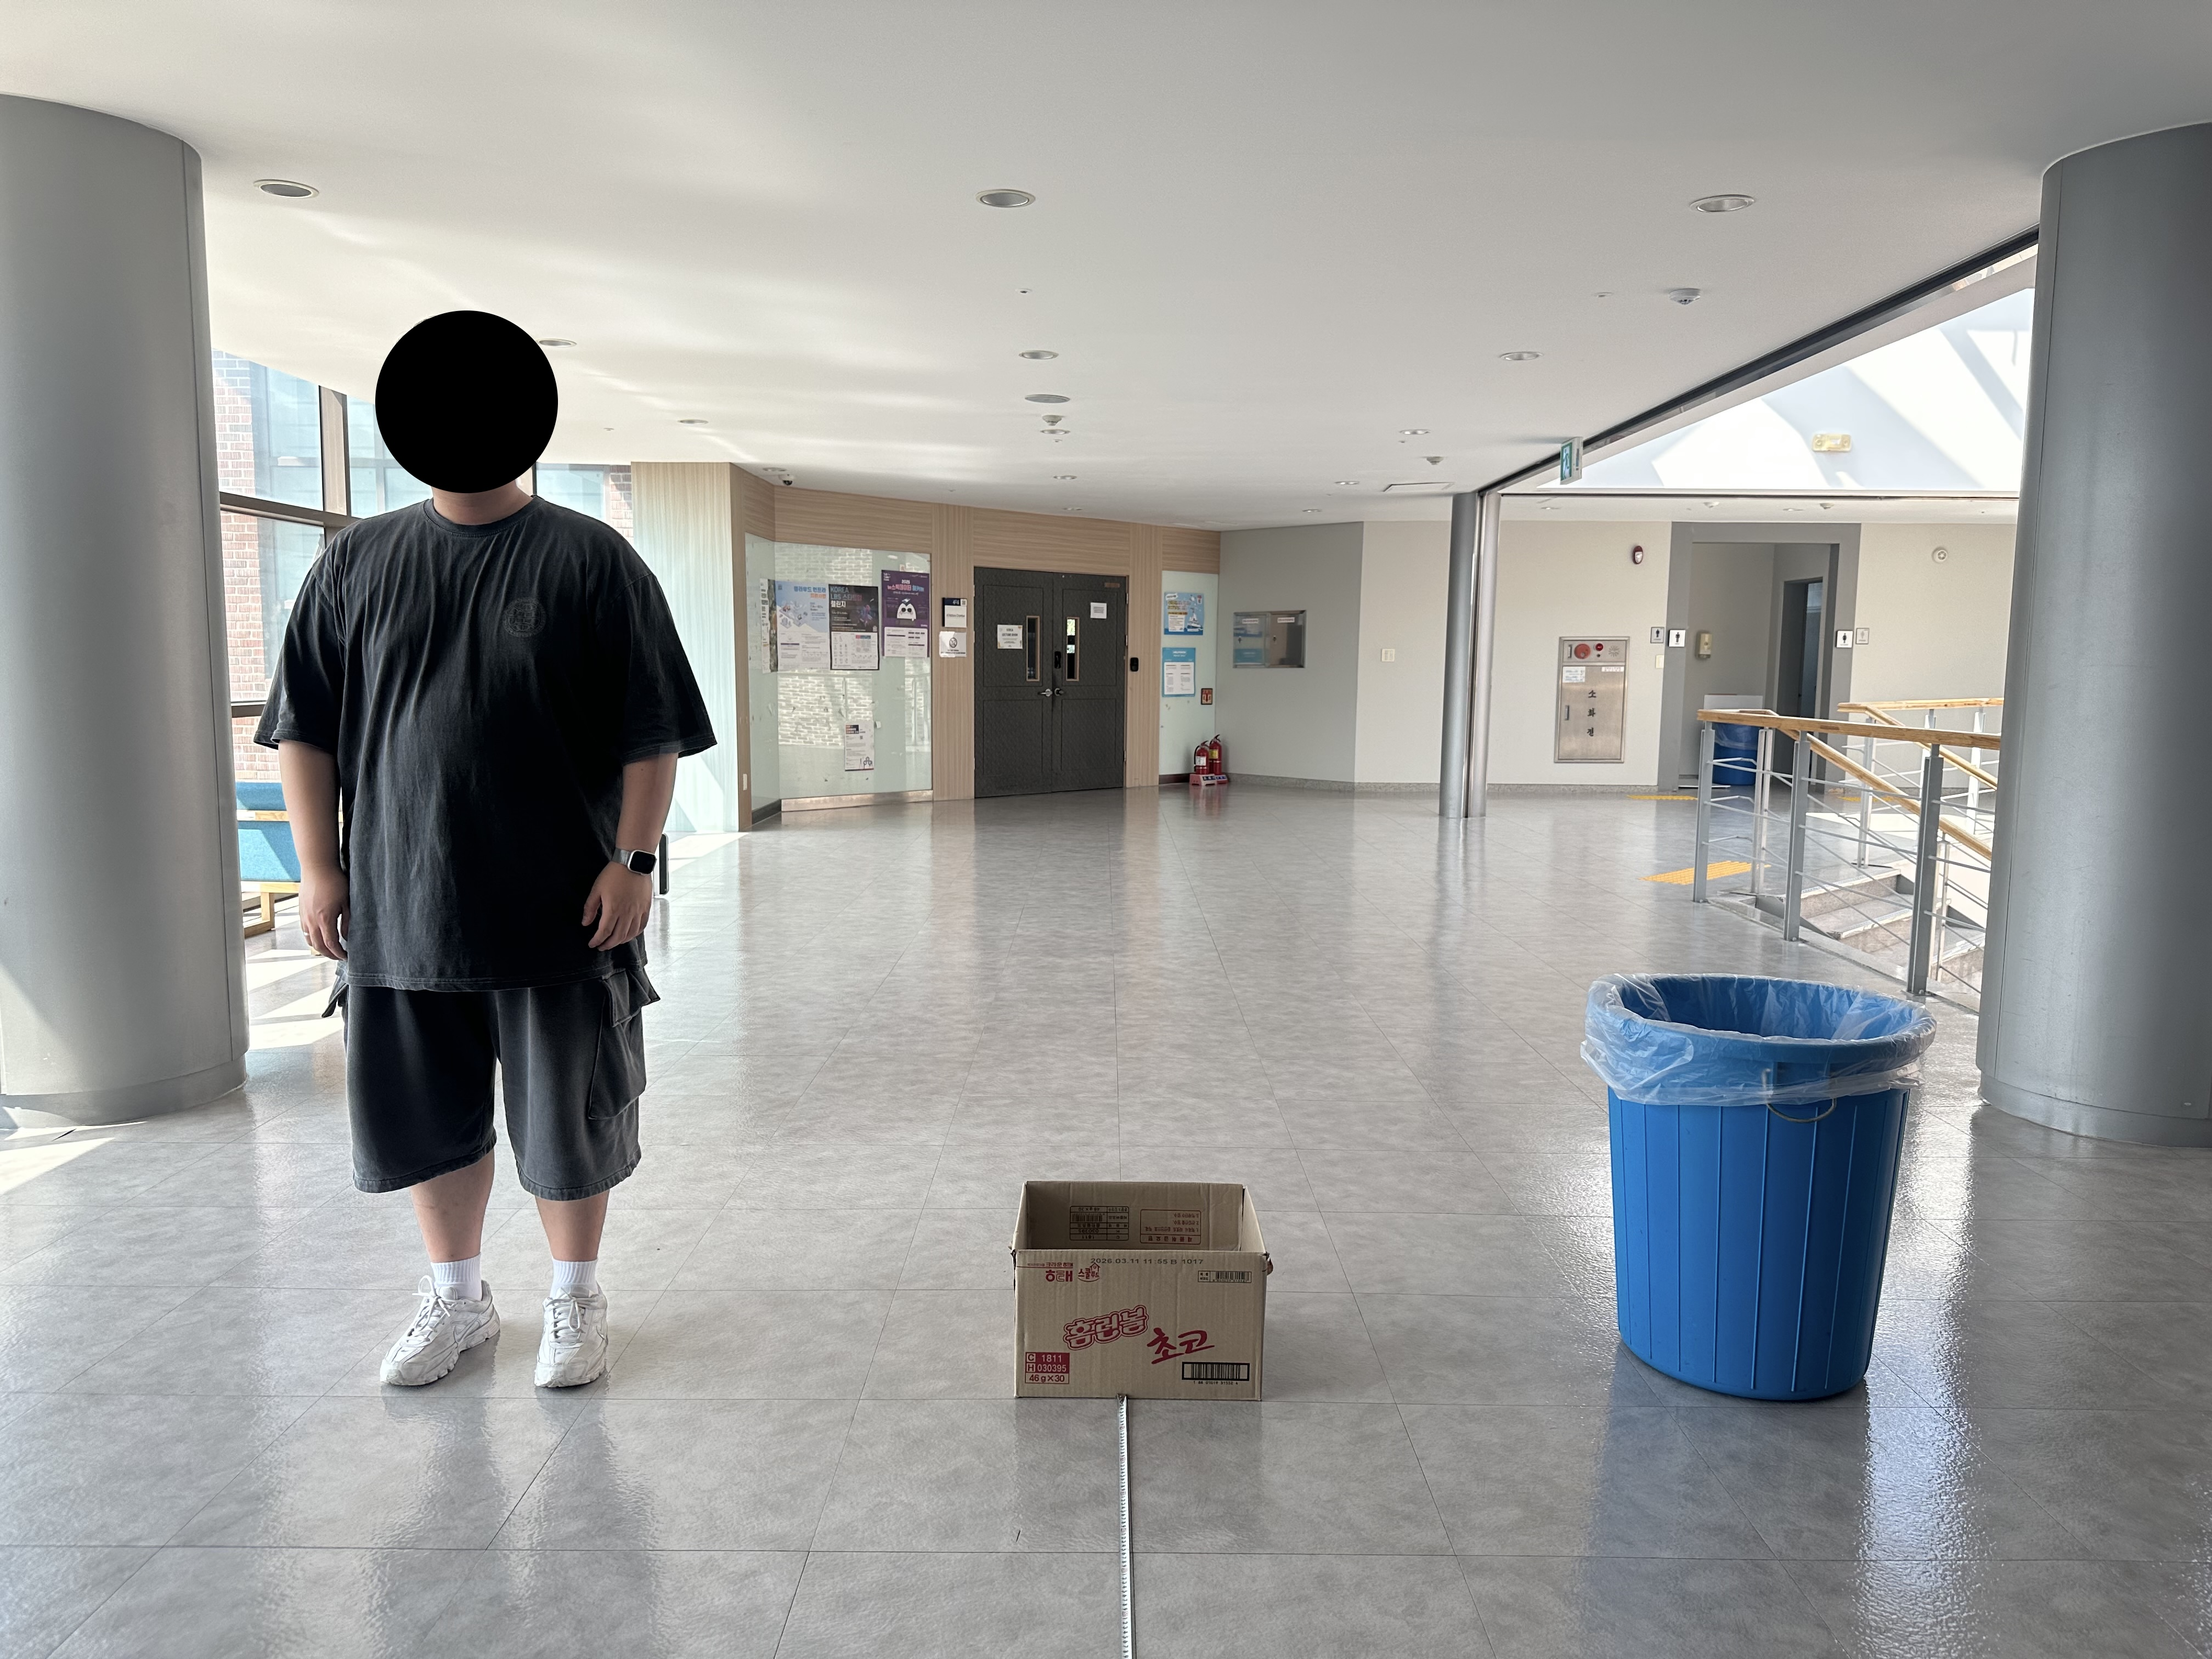
\includegraphics[width=0.92\linewidth]{experiment1_setup}
  \caption{Experimental setup for static range evaluation. Test targets are positioned at a reference distance of 2.50\,m: a person at $+20^\circ$, a cardboard box at $0^\circ$, and a cylindrical trash can at $-20^\circ$.}
  \label{fig:exp1_setup}
\end{figure}

\begin{figure}[t]
  \centering
  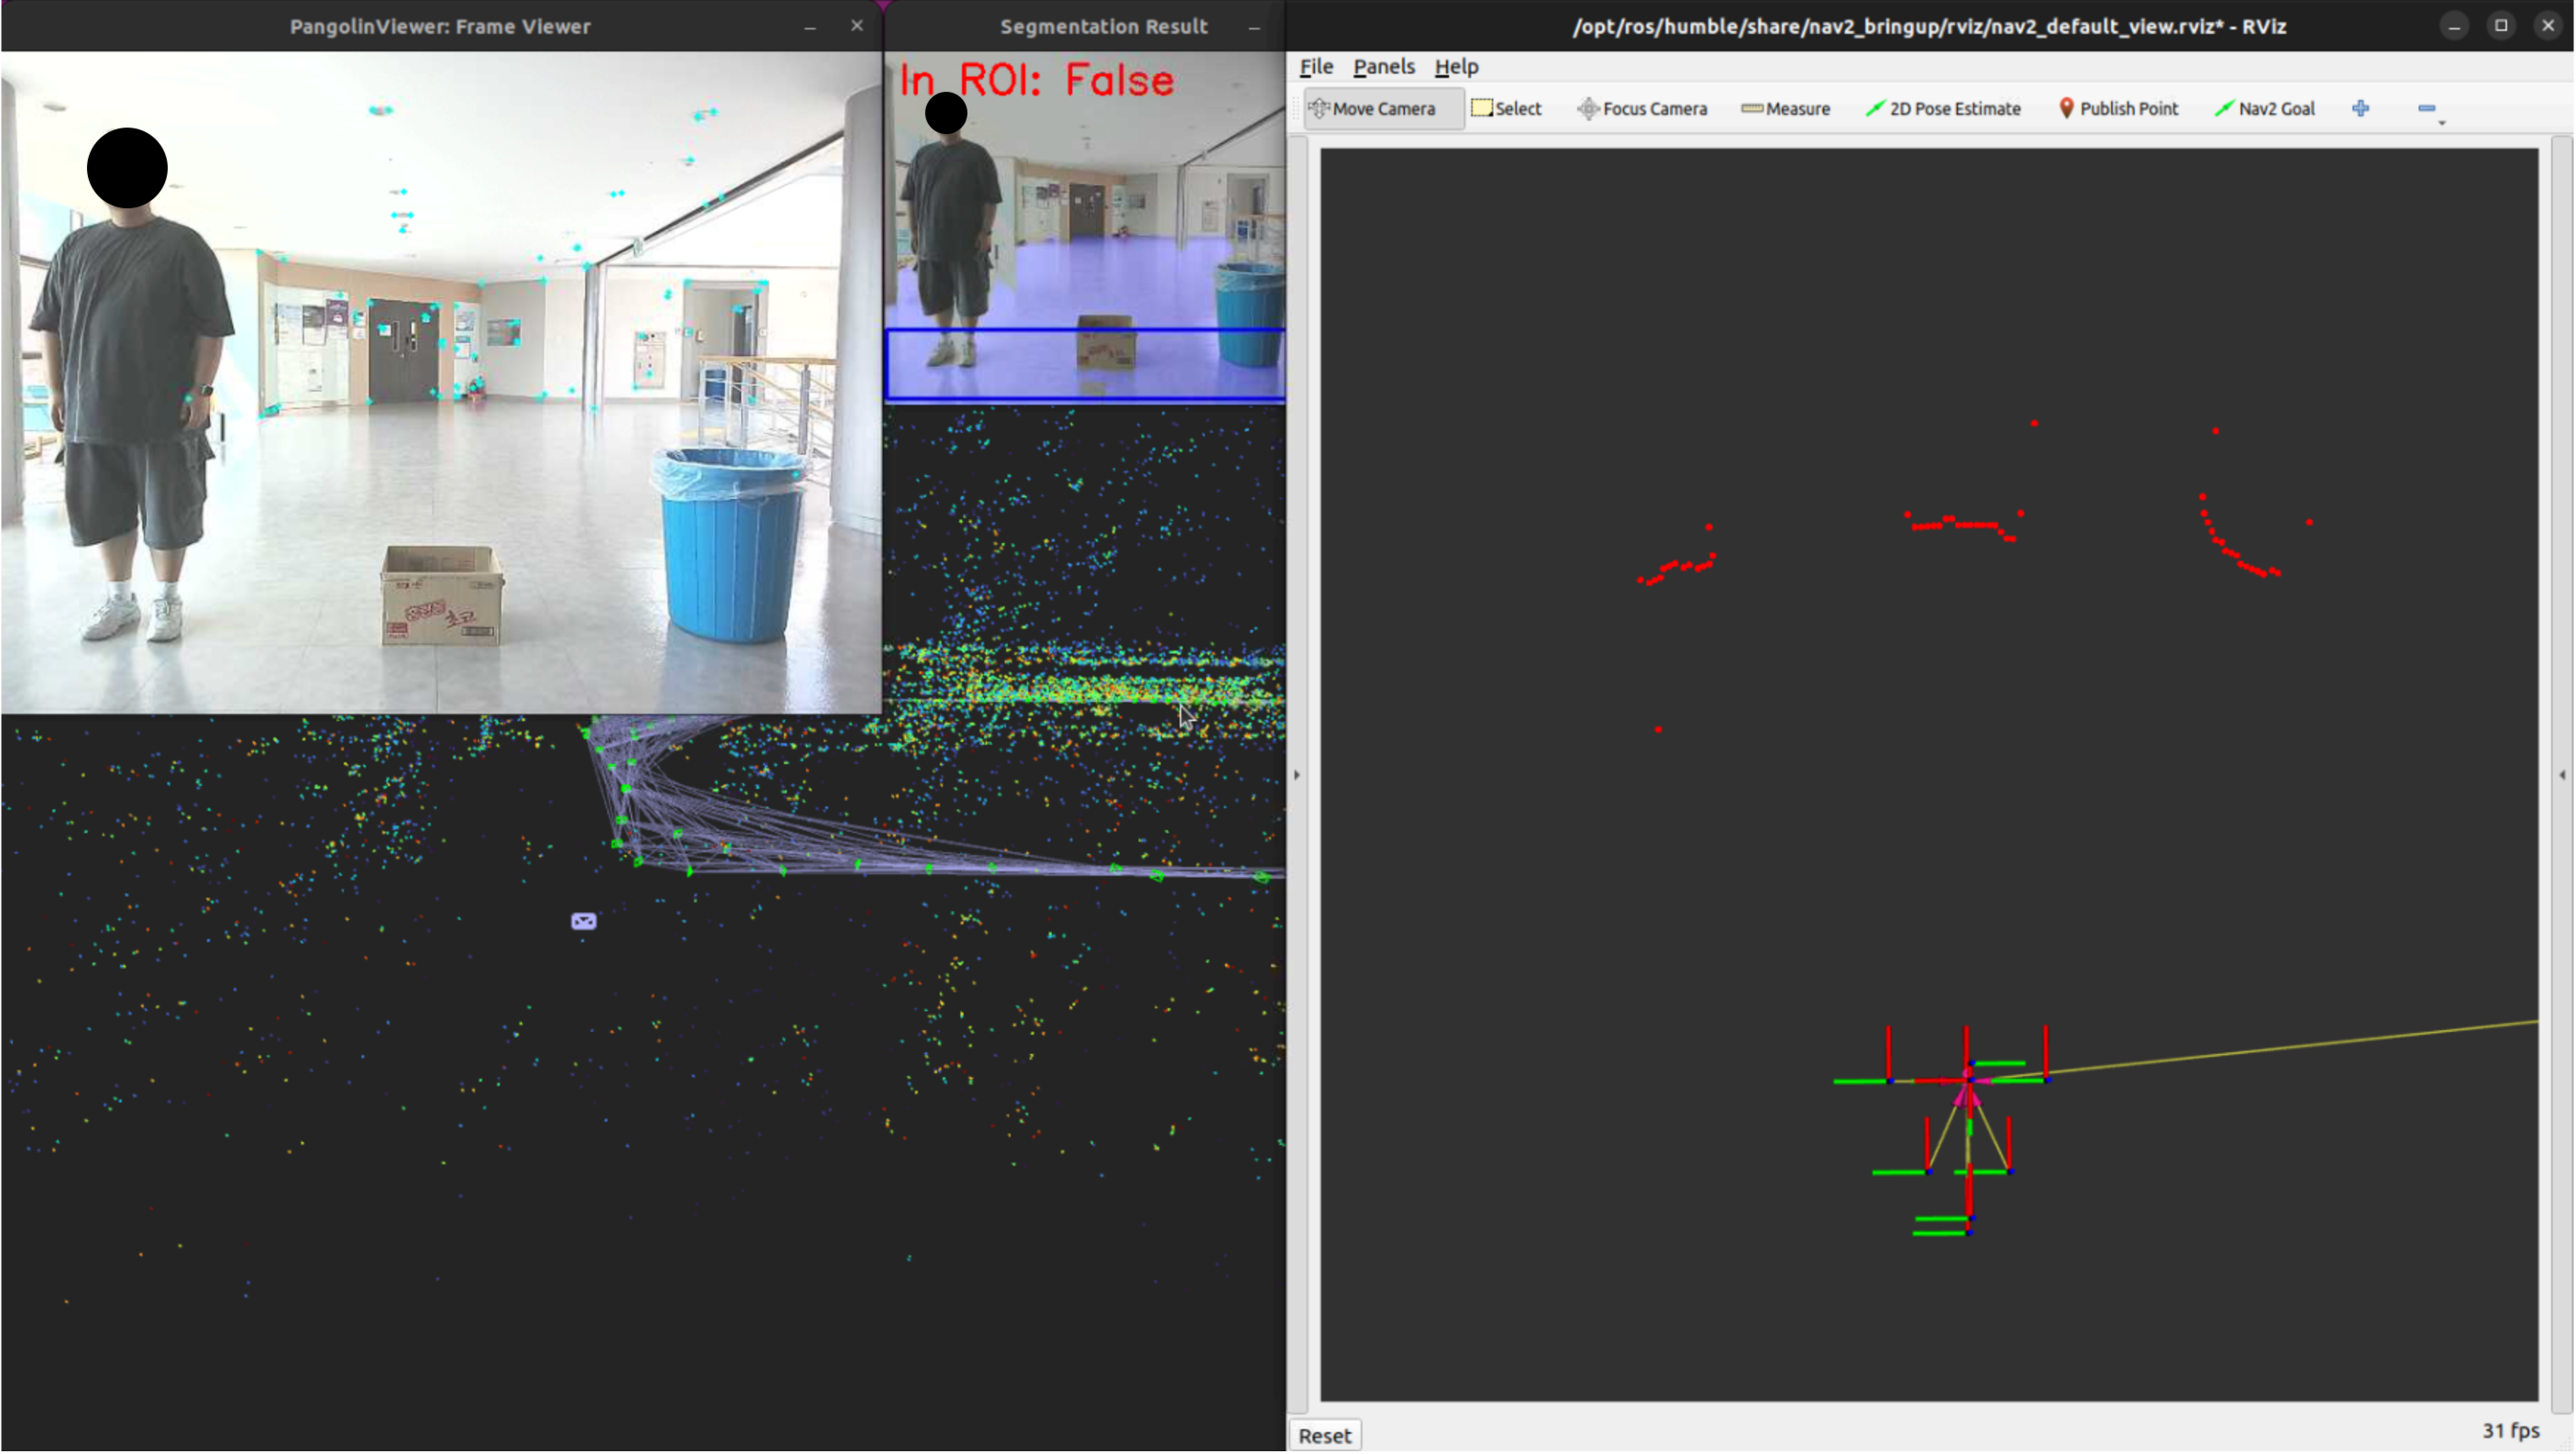
\includegraphics[width=0.92\linewidth]{live_view}
  \caption{Real-time GUI monitoring during experimental trials. The top-left panel displays raw RGB input, the top-right panel shows the segmented floor mask overlay with ROI bounding, and the bottom panel visualizes the real-time generated 141-channel LaserScan.}
  \label{fig:live_view}
\end{figure}

\begin{figure*}[!t]
  \centering
  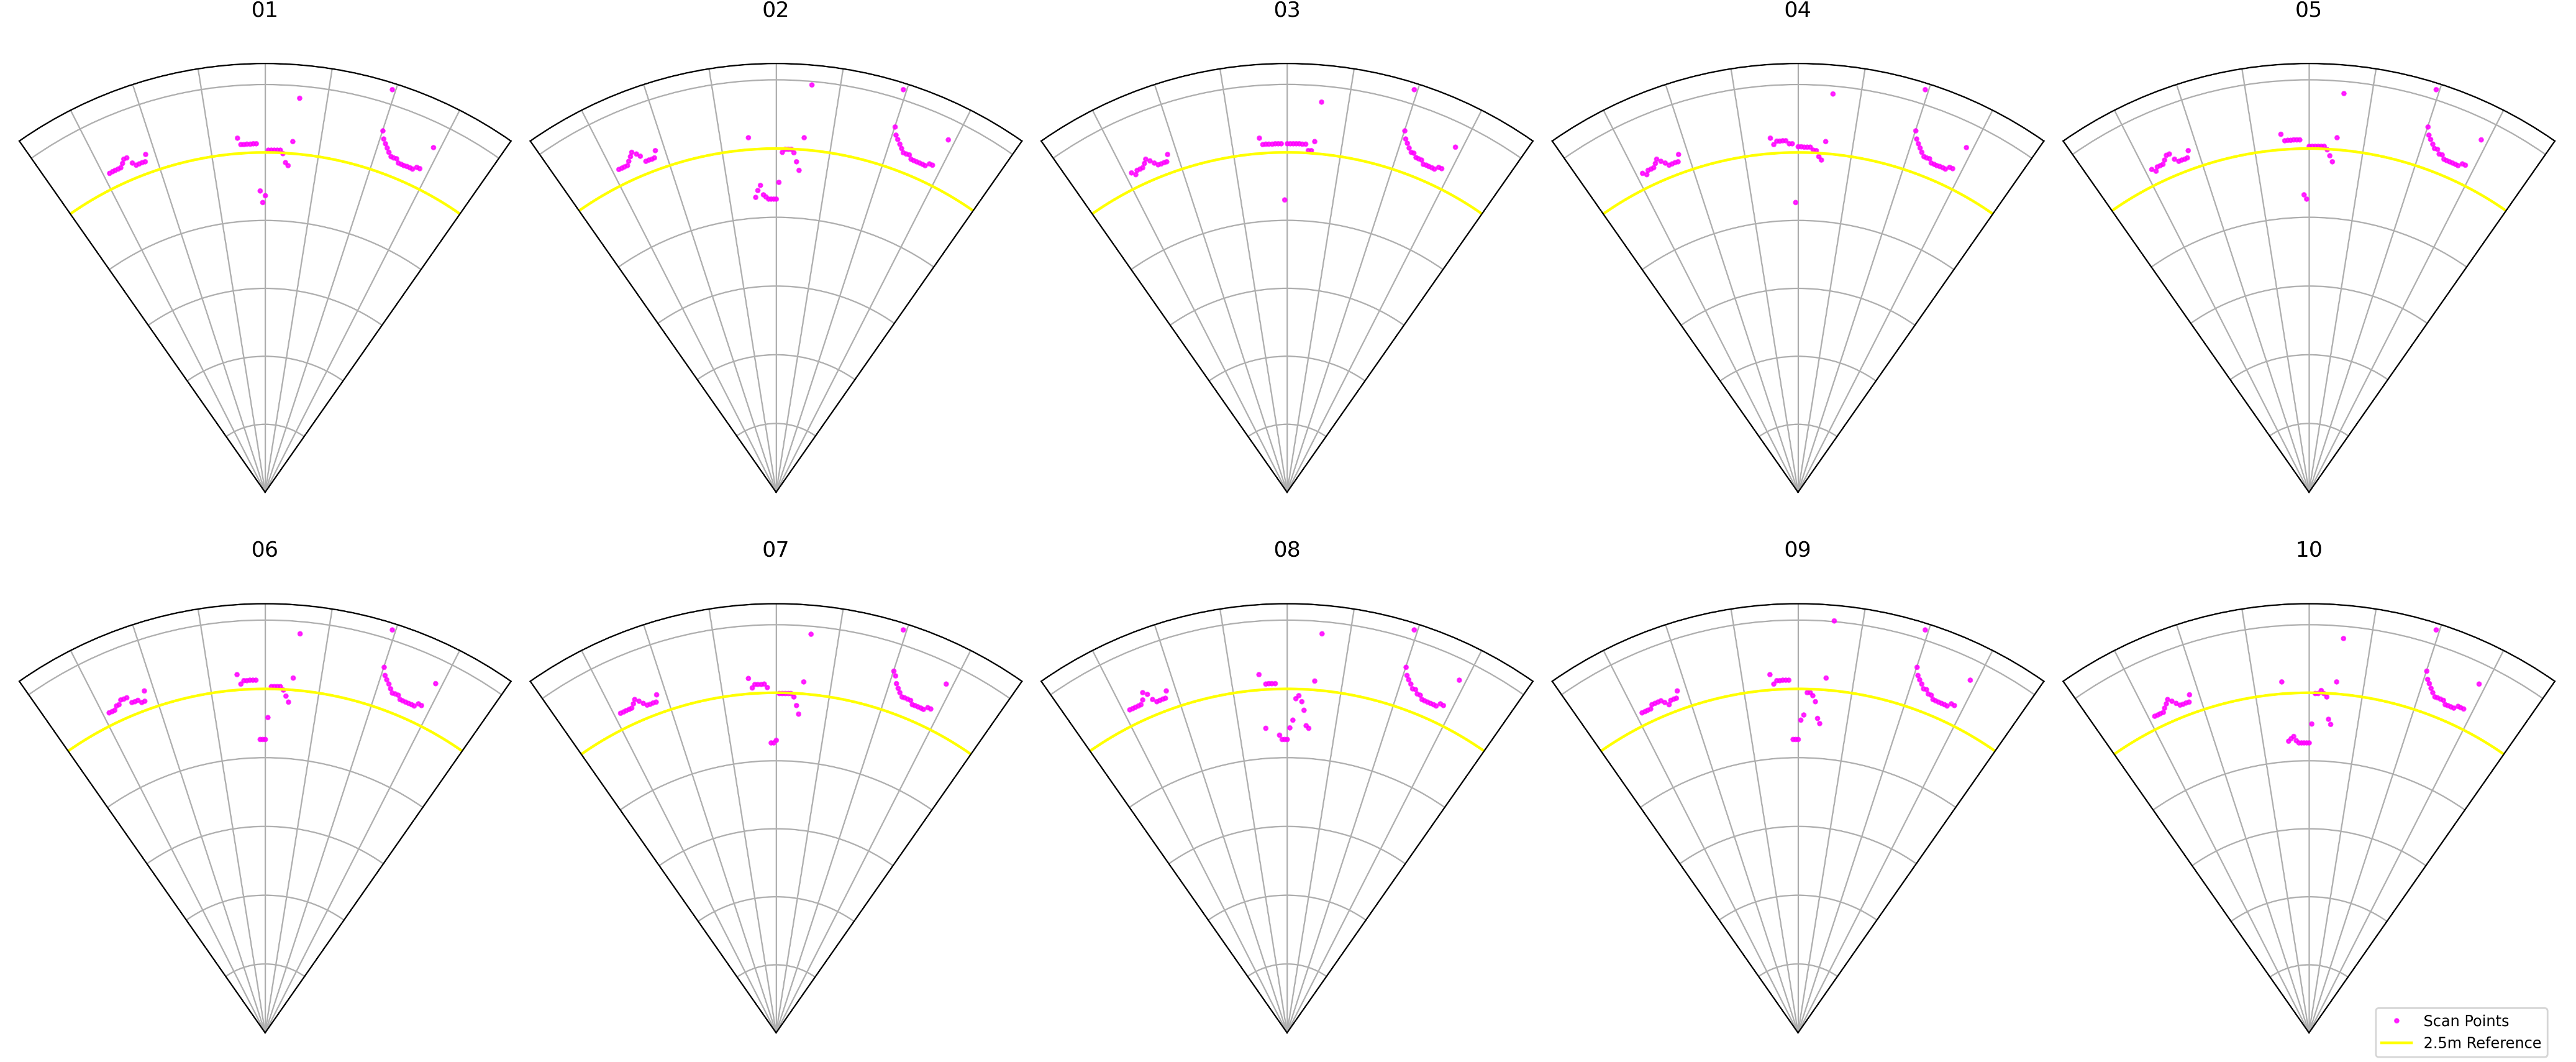
\includegraphics[width=0.92\textwidth]{experiment1_results}
  \caption{Static range estimation results across 25 consecutive frames for each target condition at 2.50\,m reference distance. Magenta markers represent virtual scan measurements; solid red lines indicate the 2.50\,m ground truth.}
  \label{fig:exp1_results}
\end{figure*}

\begin{table}[t]
  \centering
  \caption{Quantitative Static Range Precision Results at 2.50\,m Reference Distance}
  \label{tab:exp1_results}
  \resizebox{\columnwidth}{!}{%
  \begin{tabular}{lcccccc}
    \toprule
    Target Condition & Angle & Frames ($N$) & Mean Distance (m) & Std. Dev. (m) & Mean Error (m) & Relative Error (\%) \\
    \midrule
    Front (Noisy Floor) & $0^\circ$ & 25 & 2.239 & 0.172 & $-0.261$ & $-10.44\%$ \\
    Front (Clean Floor) & $0^\circ$ & 25 & 2.718 & 0.008 & $+0.218$ & $+8.72\%$ \\
    Left (Standing Adult) & $+20^\circ$ & 25 & 2.583 & 0.011 & $+0.083$ & $+3.32\%$ \\
    Right (Cylindrical Can) & $-20^\circ$ & 25 & 2.663 & 0.000 & $+0.163$ & $+6.52\%$ \\
    \bottomrule
  \end{tabular}%
  }
\end{table}

\subsubsection{Setup}
As illustrated in Fig.~\ref{fig:exp1_setup}, the physical robot was stationed on a structured indoor testing hall floor. Target obstacles were positioned at a ground-truth distance of $2.50$\,m ($\pm0.01$\,m measured by metric laser tape) at three discrete azimuth angles:
\begin{itemize}
  \item \textbf{Center ($0^\circ$)}: A rectangular cardboard box ($0.42 \times 0.34 \times 0.26$\,m).
  \item \textbf{Left ($+20^\circ$)}: An adult male pedestrian ($1.78$\,m tall).
  \item \textbf{Right ($-20^\circ$)}: A dark cylindrical receptacle ($0.63 \times 0.63 \times 0.75$\,m).
\end{itemize}
For each target condition, 25 consecutive scan frames were recorded over a 45-second duration. Live system execution is depicted in Fig.~\ref{fig:live_view}.

\subsubsection{Results and Analysis}
Table~\ref{tab:exp1_results} and Fig.~\ref{fig:exp1_results} summarize the measurement metrics. In the clean frontal condition, the system estimated a mean distance of 2.718\,m with a standard deviation of 0.008\,m (error $+0.218$\,m). Lateral targets exhibited errors of $+0.083$\,m ($+20^\circ$) and $+0.163$\,m ($-20^\circ$). Under unmitigated specular glare (noisy floor), ground reflections caused the contact line to shift forward, yielding an error of $-0.261$\,m and higher standard deviation (0.172\,m). Overall, the absolute ranging error remained bounded within 0.261\,m, demonstrating that while the virtual scan is not suited for millimeter-level metrology, it provides coarse proximity cues adequate for local reactive path planning.

\subsubsection{Target Geometry and Material Diversity Analysis}
To evaluate ranging robustness across varied geometries and materials, the static ranging benchmark was conducted across three distinct obstacle classes representing realistic indoor hazards:
\begin{enumerate}
  \item \textbf{Planar Cardboard Box ($0^\circ$, Center)}: Dimensions $0.42 \times 0.34 \times 0.26$\,m, featuring matte brown cardboard with orthogonal flat edges. Under clean floor conditions, the estimated distance was $2.718 \pm 0.008$\,m (error $+0.218$\,m, $+8.72\%$).
  \item \textbf{Standing Adult Pedestrian ($+20^\circ$, Left)}: A $1.78$\,m tall male adult wearing dark denim trousers and athletic shoes, presenting non-rigid, irregular organic contours and fabric scattering. Despite non-planar contact points, the system achieved exceptional precision with a mean distance of $2.583 \pm 0.011$\,m (error $+0.083$\,m, $+3.32\%$).
  \item \textbf{Cylindrical Trash Receptacle ($-20^\circ$, Right)}: Dimensions $0.63 \times 0.63 \times 0.75$\,m, featuring curved dark plastic with specular highlights. The system estimated $2.663 \pm 0.000$\,m (error $+0.163$\,m, $+6.52\%$).
\end{enumerate}
Across all target geometries, distance error remained within $0.261$\,m. The low standard deviations ($\sigma \le 0.011$\,m under normal lighting) verify that the 2D Euclidean LUT accurately accounts for lateral angular ray expansion at non-zero azimuth angles ($\pm 20^\circ$).

\subsection{Experiment 2: Closed-Loop Autonomous Obstacle Avoidance under Monocular Nav2 Navigation}
\label{subsec:exp2}

\begin{figure}[t]
  \centering
  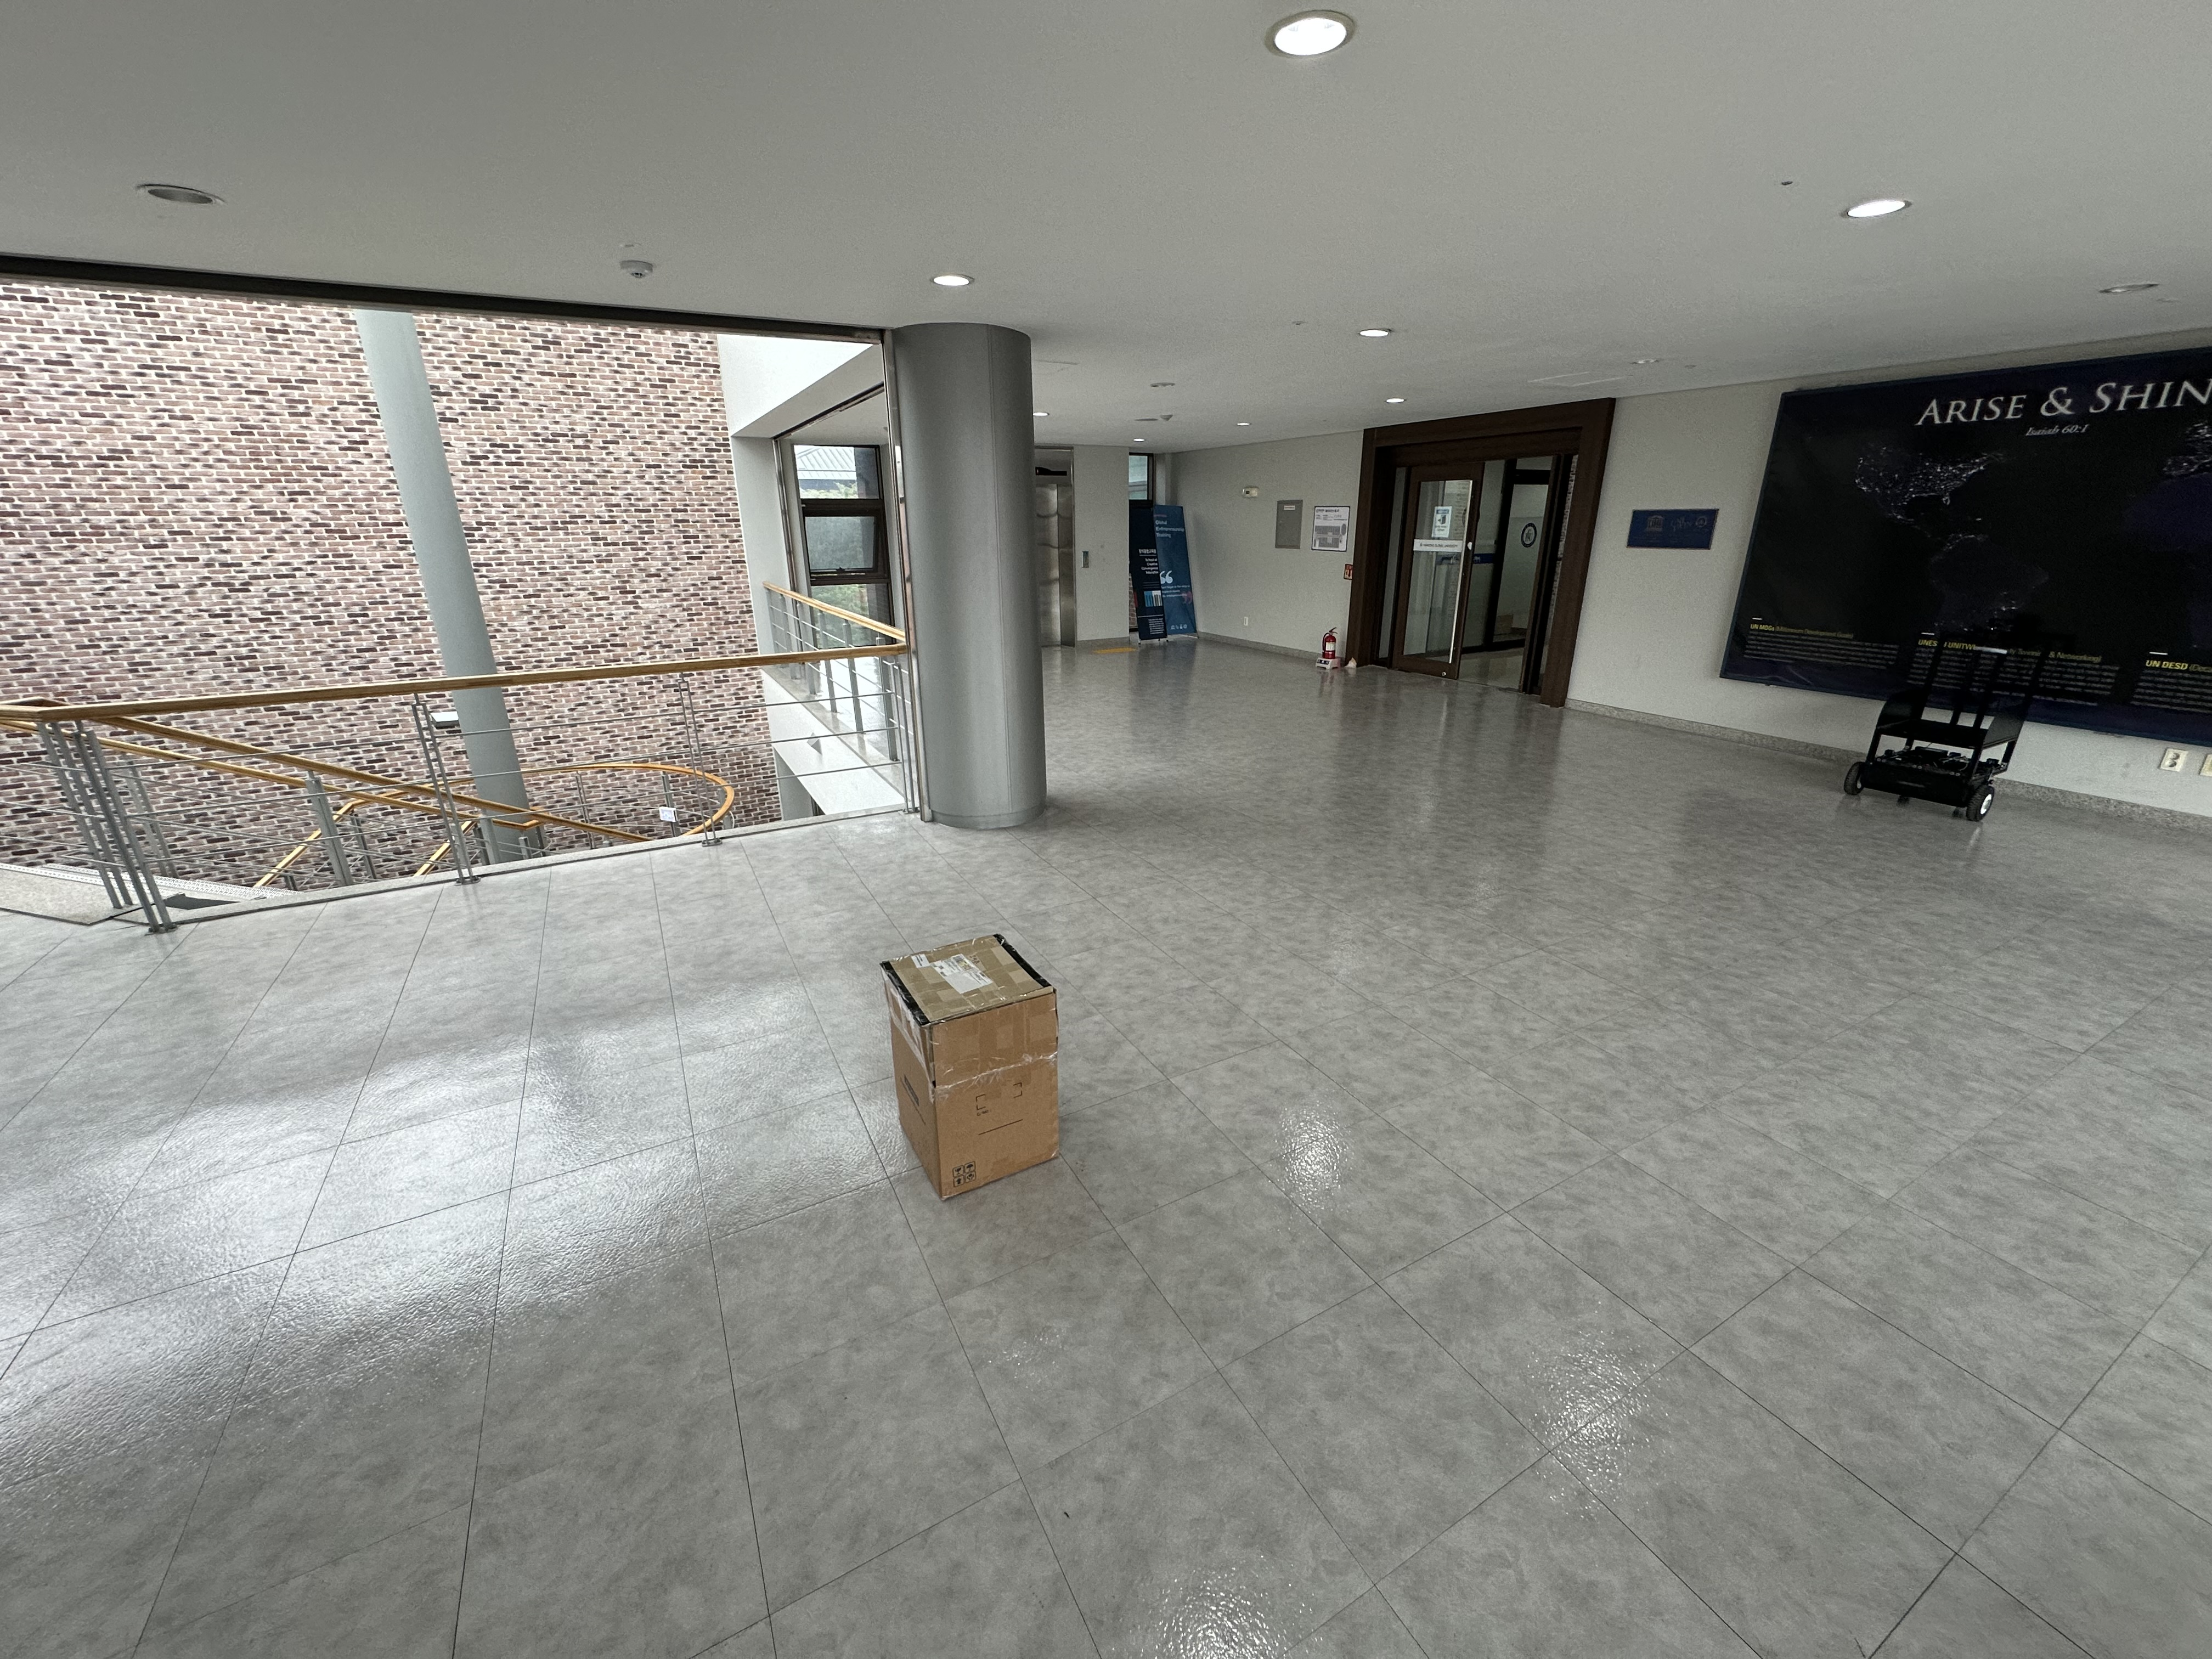
\includegraphics[width=0.88\linewidth]{experiment2_setup}
  \caption{Real-world test arena for closed-loop autonomous obstacle avoidance. The OMO-R1 mobile robot (background right) navigates along a 10.0-meter trajectory facing a stationary cardboard box obstacle ($0.40 \times 0.40 \times 0.50$\,m) positioned at $X \approx 4.0\text{--}4.5$\,m on glossy, reflective floor tiles.}
  \label{fig:exp2_setup}
\end{figure}

\begin{figure*}[!t]
  \centering
  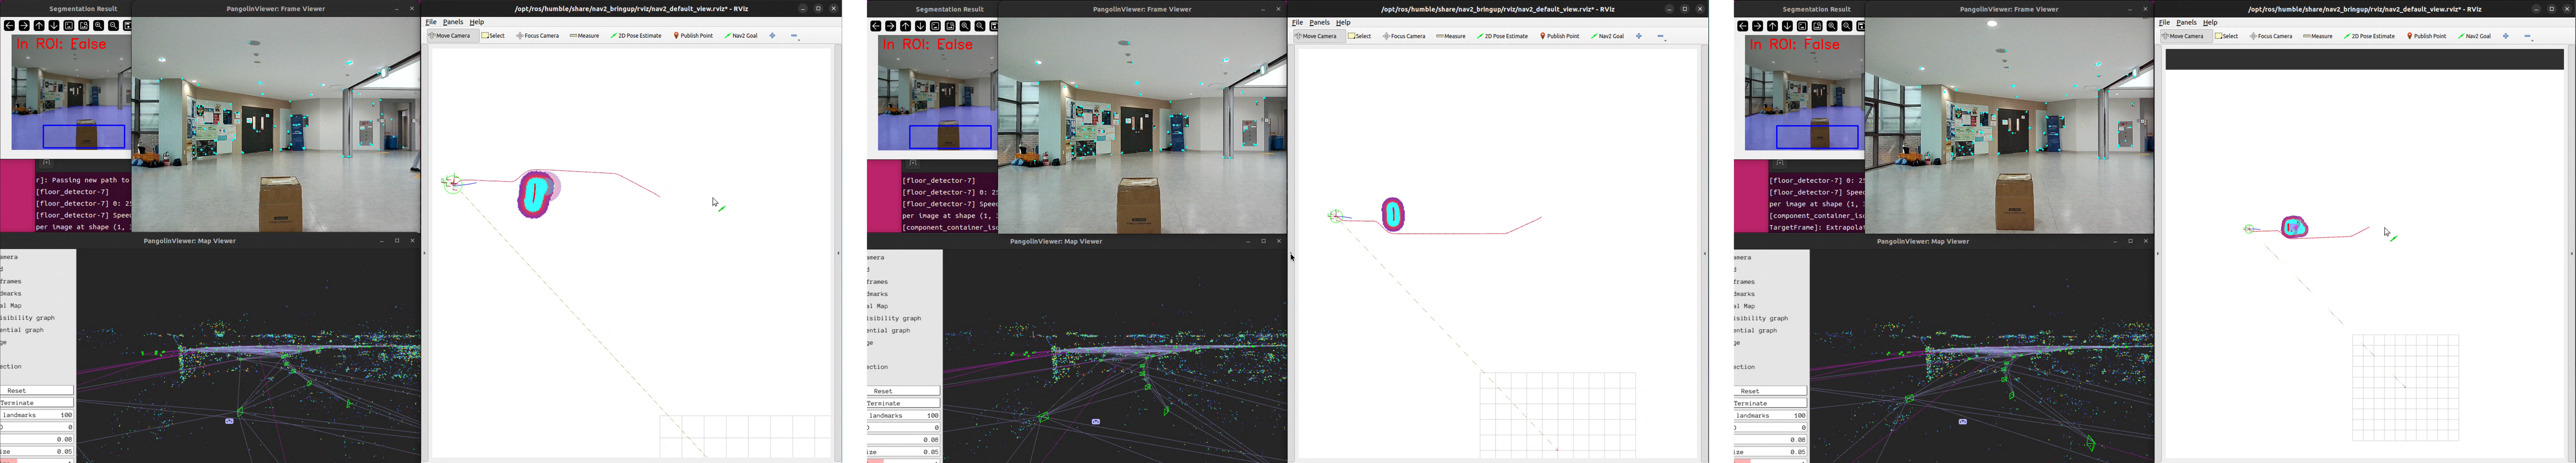
\includegraphics[width=0.94\textwidth]{nav2_obstacle_avoidance_sequence}
  \caption{Sequential real-world execution of autonomous obstacle avoidance: (a) robot approaches obstacle while marking costmap, (b) global and local planners generate lateral swerve maneuver to bypass obstacle, and (c) robot re-aligns toward the 10.0-meter terminal goal. (Note: Auxiliary PangolinViewer windows in recordings were for offline logging; online Nav2 costmap marking and avoidance strictly operated on V-LiDAR LaserScan without SLAM map feedback.)}
  \label{fig:exp2_sequence}
\end{figure*}

\begin{table*}[!t]
  \centering
  \caption{Full Quantitative Results Across 20 Consecutive Real-World Obstacle Avoidance Trials (Mean $\pm$ SD metrics computed across the 18 successfully completed runs)}
  \label{tab:exp2_results}
  \begin{tabularx}{\textwidth}{lcccccX}
    \toprule
    Run Index & Motion Time (s) & Travel $X$ (m) & Lat. Swerve $Y$ (m) & Min Range (m) & Max $\omega_z$ (rad/s) & Nav Outcome \\
    \midrule
    \texttt{run01} & 44.2 & 9.76 & 0.958 & 2.178 & 0.200 & Successfully avoided and completed \\
    \texttt{run02} & 44.0 & 9.78 & 0.903 & 2.178 & 0.367 & Successfully avoided and completed \\
    \texttt{run03} & 71.2 & 9.77 & 1.056 & 2.178 & 0.267 & Successfully avoided and completed \\
    \texttt{run04} & 41.3 & 9.77 & 0.887 & 2.385 & 0.133 & Successfully avoided and completed \\
    \texttt{run05} & 38.8 & 9.76 & 1.362 & 2.429 & 0.267 & Successfully avoided and completed \\
    \texttt{run06} & 53.9 & 9.77 & 1.124 & 2.178 & 0.400 & Successfully avoided and completed \\
    \texttt{run07} & 50.5 & 9.78 & 0.942 & 2.187 & 0.467 & Successfully avoided and completed \\
    \texttt{run08} & 110.9 & \textbf{3.70} & 0.899 & 2.413 & 0.200 & Halted near obstacle ($X=3.70$\,m) \\
    \texttt{run09} & 39.5 & 9.78 & 0.980 & 2.178 & 0.200 & Successfully avoided and completed \\
    \texttt{run10} & 52.9 & 9.76 & 1.928 & 2.178 & 0.500 & Successfully avoided and completed \\
    \texttt{run11} & 54.7 & 9.76 & 0.989 & 2.178 & 0.333 & Successfully avoided and completed \\
    \texttt{run12} & 74.0 & \textbf{2.91} & 1.069 & 2.218 & 0.333 & Halted near obstacle ($X=2.91$\,m) \\
    \texttt{run13} & 44.2 & 9.78 & 1.274 & 2.313 & 0.300 & Successfully avoided and completed \\
    \texttt{run14} & 41.9 & 9.82 & 2.563 & 2.277 & 0.400 & Successfully avoided and completed \\
    \texttt{run15} & 43.1 & 9.77 & 0.781 & 2.178 & 0.400 & Successfully avoided and completed \\
    \texttt{run16} & 46.8 & 9.76 & 0.987 & 2.178 & 0.347 & Successfully avoided and completed \\
    \texttt{run17} & 49.1 & 9.76 & 1.024 & 2.178 & 0.500 & Successfully avoided and completed \\
    \texttt{run18} & 48.1 & 9.76 & 0.828 & 2.179 & 0.500 & Successfully avoided and completed \\
    \texttt{run19} & 50.2 & 9.82 & 1.676 & 2.198 & 0.500 & Successfully avoided and completed \\
    \texttt{run20} & 46.2 & 9.77 & 1.702 & 2.214 & 0.500 & Successfully avoided and completed \\
    \midrule
    \textbf{Mean $\pm$ SD} & \textbf{47.8 $\pm$ 7.3\,s} & \textbf{9.77 $\pm$ 0.02\,m} & \textbf{1.22 $\pm$ 0.45\,m} & \textbf{2.22 $\pm$ 0.08\,m} & \textbf{0.36 $\pm$ 0.12\,rad/s} & \textbf{Success Rate: 18/20 (90.0\%)} \\
    \bottomrule
  \end{tabularx}
\end{table*}

\subsubsection{Setup}
To evaluate closed-loop obstacle avoidance, the pipeline was deployed on an OMO-R1 mobile robot ($r_{\mathrm{robot}} = 0.33$\,m, footprint radius 0.40\,m) equipped with an Intel Core Ultra 7 155H CPU (Ubuntu 22.04, ROS 2 Humble) and a forward camera ($h=1.05$\,m, $\gamma=2.0^\circ$).

As shown in Fig.~\ref{fig:exp2_setup}, a straight 10.0-meter relative goal ($(X, Y) = (10.0, 0.0)$\,m) was commanded without a pre-built static occupancy map. A cardboard box obstacle ($0.40 \times 0.40 \times 0.50$\,m) was positioned at $X \approx 4.0\text{--}4.5$\,m along the centerline. Calibrated wheel odometry tracked relative motion, while synthesized LaserScan was ingested into the Nav2 local costmap for mapless reactive avoidance. While calibrated odometry reliably evaluates evasive clearance and goal progress, it remains subject to minor wheel slip during swerves without external MoCap. The robot autonomously detected the obstacle, replanned, and completed 20 consecutive trials.

\subsubsection{Quantitative Avoidance Performance}
Table~\ref{tab:exp2_results} provides the quantitative trajectory metrics across all 20 runs. The navigation outcomes demonstrate:
\begin{itemize}
  \item \textbf{Task Completion Rate}: The robot completed 18 of the 20 trials without intervention (\textbf{90.0\% success rate}), demonstrating a promising goal completion rate under static single-obstacle test scenarios.
  \item \textbf{Consistent Lateral Avoidance}: In the 18 successful runs, evasive steering initiated at range $2.22 \pm 0.08$\,m, swerving laterally by $Y = 1.22 \pm 0.45$\,m ($0.78\text{--}2.56$\,m) before converging back to the goal.
  \item \textbf{Rhythmic Velocity Execution}: Pure motion duration for completed trials averaged $47.8 \pm 7.3$\,s (total recording duration $58.1 \pm 9.3$\,s), corresponding to an effective cruising speed of $\sim0.22\,\text{m/s}$ ($v_{\max} = 0.30\,\text{m/s}$).
  \item \textbf{Lower-Bounded Minimum Range}: Consistent with the theoretical derivation in Section~\ref{sec:blind_spot}, the minimum recorded distance in Table~\ref{tab:exp2_results} consistently reached a lower bound of 2.178\,m.
\end{itemize}

Fig.~\ref{fig:exp2_sequence} depicts a representative avoidance sequence. As shown in telemetry windows, the obstacle is detected at $\sim 4$\,m, marked in the local costmap, and circumvented smoothly by Nav2 without 3D SLAM maps.

\subsection{Comparative Evaluation Against Monocular Depth Baselines}
\label{subsec:baseline_benchmark}

A fundamental research question in monocular robot perception is whether specialized floor segmentation offers tangible operational advantages over general-purpose Monocular Depth Estimation (MDE) networks. To establish a rigorous empirical baseline under actual robotic operating conditions, we deployed two leading open-source MDE models alongside the proposed V-LiDAR across 200 consecutive synchronized sensor frames recorded during real-world autonomous navigation trials (\texttt{vlidar\_run01} and \texttt{vlidar\_run02}) on the identical onboard mobile robot hardware (Intel Core Ultra 7 155H CPU, 16 cores, 22 threads, 32\,GB RAM):
\begin{enumerate}
  \item \textbf{MiDaS v2.1 Small}~\cite{ranftl_2020_towards}: A lightweight, convolutional EfficientNet-based depth estimation model designed for resource-constrained devices.
  \item \textbf{Depth Anything V2 Small}~\cite{yang_2024_depth}: A state-of-the-art vision transformer (DINOv2-ViT) foundation model trained on large-scale synthetic and real datasets.
\end{enumerate}

To extract planar range scans from dense depth predictions, depth maps were converted to 2D range scans along the camera centerline using standard pinhole reprojection. Because foundation MDE models output scale- and shift-invariant relative disparity rather than absolute metric depth, an explicit scale recovery step is mandatory for fair spatial comparison. We aligned each predicted relative disparity map $d_{\mathrm{rel}}$ to metric meters via linear affine calibration: $d_{\mathrm{metric}} = (s \cdot d_{\mathrm{rel}} + t)^{-1}$, where parameters $(s, t)$ were optimally fitted using ground-truth reference distances obtained from stationary calibration frames. Table~\ref{tab:baseline_benchmark} summarizes the architectural, computational, and dynamic ranging comparisons across the 200 synchronized frames.

\begin{table*}[!t]
  \centering
  \footnotesize
  \caption{Quantitative Benchmark: Proposed V-LiDAR vs. Monocular Depth Estimation (MDE) Baselines on Onboard CPU (Intel Core Ultra 7 155H)}
  \label{tab:baseline_benchmark}
  \resizebox{\textwidth}{!}{%
  \begin{tabular}{llcccccc}
    \toprule
    Perception Model & Architecture / Backend & Parameters & Disk Size & Latency (ms) & Throughput & Dynamic MAE & Real-Time (10\,Hz)? \\
    \midrule
    \textbf{V-LiDAR (Proposed)} & \textbf{OpenVINO FP16 (Intel CPU)} & \textbf{2.84\,M} & \textbf{5.4\,MB} & \textbf{12.9 $\pm$ 1.9} & \textbf{78.4\,FPS} & \textbf{0.192\,m} & \textbf{Yes (7.7$\times$ margin)} \\
    \textbf{MiDaS v2.1 Small} & PyTorch CPU (EfficientNet MDE) & 21.3\,M & 42.0\,MB & 42.9 $\pm$ 7.4 & 23.3\,FPS & 0.880\,m & Marginally (2.3$\times$ margin) \\
    \textbf{Depth Anything V2 Small} & PyTorch CPU (DINOv2-ViT MDE) & 24.8\,M & 97.5\,MB & 601.4 $\pm$ 26.5 & 1.7\,FPS & 3.298\,m & \textbf{No (Fails by 6.0$\times$)} \\
    \bottomrule
  \end{tabular}%
  }
\end{table*}

As detailed in Table~\ref{tab:baseline_benchmark}, V-LiDAR accelerated by OpenVINO FP16 requires only $12.9$\,ms per frame ($78.4$\,FPS). Even in vanilla PyTorch CPU, V-LiDAR achieves $50.7$\,FPS ($19.7 \pm 18.3$\,ms), outperforming MiDaS ($23.3$\,FPS) by $2.2\times$ and Depth Anything V2 ($1.7$\,FPS, $601.4$\,ms) by $29.8\times$ ($46.6\times$ with OpenVINO). Critically, foundation MDE models suffer prohibitive computational latency: Depth Anything V2 requires $601.4 \pm 26.5$\,ms per frame on edge CPU, breaching Nav2's 10\,Hz control deadline by $6.0\times$. Furthermore, dynamic viewpoint shifts induce unmodeled scale drift and boundary bleeding along the floor interface, yielding approach MAEs of $0.880$\,m (MiDaS) and $3.298$\,m (Depth Anything V2). In contrast, V-LiDAR deterministically resolves metric scale via calibrated 2D ground geometry, eliminating scale ambiguity while maintaining a bounded $0.192$\,m MAE with only 2.84\,M parameters.

\subsection{Component Ablation Study on Artifact Suppression}
\label{subsec:ablation_study}

To isolate each module's algorithmic impact under identical conditions and eliminate physical trajectory stochasticity, the ablation study was conducted via Software-in-the-Loop (SIL) offline replay across synchronized multi-run rosbags ($>6{,}000$ frames across the 20 navigation trials). Replaying through Nav2's local costmap and DWB planner evaluated five progressive configurations:
\begin{enumerate}
  \item \textbf{(A) Base Model}: Standalone YOLOv11n-seg selecting only the highest-confidence floor mask ($m_0$) paired with a 1D row-to-distance lookup table.
  \item \textbf{(B) +Mask Merging}: Incorporating element-wise bitwise-OR aggregation across all $K$ detected floor instances ($\bigvee_{k=1}^K m_k$).
  \item \textbf{(C) +Morphological Closing}: Adding the $7 \times 7$ rectangular closing kernel (two iterations) to bridge reflection-induced dark holes.
  \item \textbf{(D) +Temporal Filtering}: Introducing the asymmetric EMA ($\alpha=0.6$) and bidirectional persistence ($N_{\mathrm{onset}}=2, N_{\mathrm{clear}}=2$) filter.
  \item \textbf{(E) +OpenVINO Engine (Full Pipeline)}: Compiling configuration (D) into an OpenVINO FP16 runtime.
\end{enumerate}

\begin{table*}[!t]
  \centering
  \footnotesize
  \caption{Systematic Component Ablation Study: Quantitative Progression of Artifact Suppression (Evaluated via Software-in-the-Loop Offline Replay Across the 20 Physical Navigation Datasets)}
  \label{tab:ablation_study}
  \begin{tabularx}{\textwidth}{@{}clccccX@{}}
    \toprule
    Config & Included Modules & FPS & Jitter $\sigma$ (m) & False Obs. & Success & Primary Impact / Failure Mode \\
    \midrule
    \textbf{(A)} & Base YOLOv11n-seg + 1D LUT & 49.7 & 0.384 & 38.5\% & 60.0\% (12/20) & Floor split by obstacle occlusions; severe glare holes trigger phantom obstacles. \\
    \textbf{(B)} & (A) + Multi-Instance Bitwise-OR & 48.2 & 0.245 & 24.0\% & 70.0\% (14/20) & Recovers disjoint floor patches; eliminates artificial lateral barriers. \\
    \textbf{(C)} & (B) + $7 \times 7$ Morphological Closing & 46.5 & 0.172 & 11.2\% & 80.0\% (16/20) & Seals specular floor reflection voids up to 6 pixels wide; smooths boundary noise. \\
    \textbf{(D)} & (C) + Bidirectional Temporal EMA \& Persistence & 45.1 & \textbf{0.008} & \textbf{1.8\%} & \textbf{90.0\% (18/20)} & Suppresses transient single-frame flicker; distance jitter drops by 97.9\%. \\
    \textbf{(E)} & \textbf{(D) + OpenVINO FP16 (Full)} & \textbf{78.4} & \textbf{0.008} & \textbf{1.8\%} & \textbf{90.0\% (18/20)} & \textbf{1.74$\times$ inference speedup (12.9\,ms latency); frees CPU for Nav2 planners.} \\
    \bottomrule
    \multicolumn{7}{@{}p{\textwidth}@{}}{\footnotesize \textit{Note:} False Obs. represents the percentage of frames where specular reflections generated spurious readings ($<5.0$\,m) in clear floor sectors. Success rates across Configs (A)--(E) denote simulated completions where replayed scans were re-ingested into DWB planners to verify whether phantom obstacles induced path abortion.}
  \end{tabularx}
\end{table*}

The ablation trajectory in Table~\ref{tab:ablation_study} clearly demonstrates the cumulative performance contribution of each post-processing and acceleration module:
\begin{itemize}
  \item In Config (A), glossy floor glare induced false obstacle readings in 38.5\% of frames (see segmentation artifacts under specular glare in Fig.~\ref{fig:seg_artifact}), resulting in erratic stops and a low 60.0\% success rate.
  \item Multi-instance merging (Config B) eliminated false barriers formed when the obstacle visually bisected the floor region, increasing success to 70.0\%.
  \item Morphological closing (Config C) reduced false obstacle detections by more than half (to 11.2\%), filling dark specular reflections.
  \item Temporal persistence (Config D) virtually eliminated measurement jitter, reducing range variance $\sigma$ from $0.172$\,m to $0.008$\,m and false obstacle rates to 1.8\%, driving navigation success to \textbf{90.0\%}.
  \item Finally, OpenVINO acceleration (Config E) boosted throughput from 45.1 to 78.4\,FPS without altering spatial accuracy.
\end{itemize}

\section{Discussion and Failure Analysis}
\label{sec:discussion}

\subsection{Root Cause Analysis of the Two Failed Trials}
\label{subsec:failure_analysis}
In two of the 20 trials (\texttt{run08} at $X=3.70$\,m and \texttt{run12} at $X=2.91$\,m), the robot safely avoided physical collision with the obstacle but halted prematurely before reaching the 10.0-meter destination. An in-depth post-hoc analysis of synchronized rosbag data revealed that these halts were not caused by perception dropouts or segmentation artifacts (Fig.~\ref{fig:seg_artifact}), but rather by subtle interactions between local costmap inflation geometry and local planner critics:

\begin{figure}[t]
  \centering
  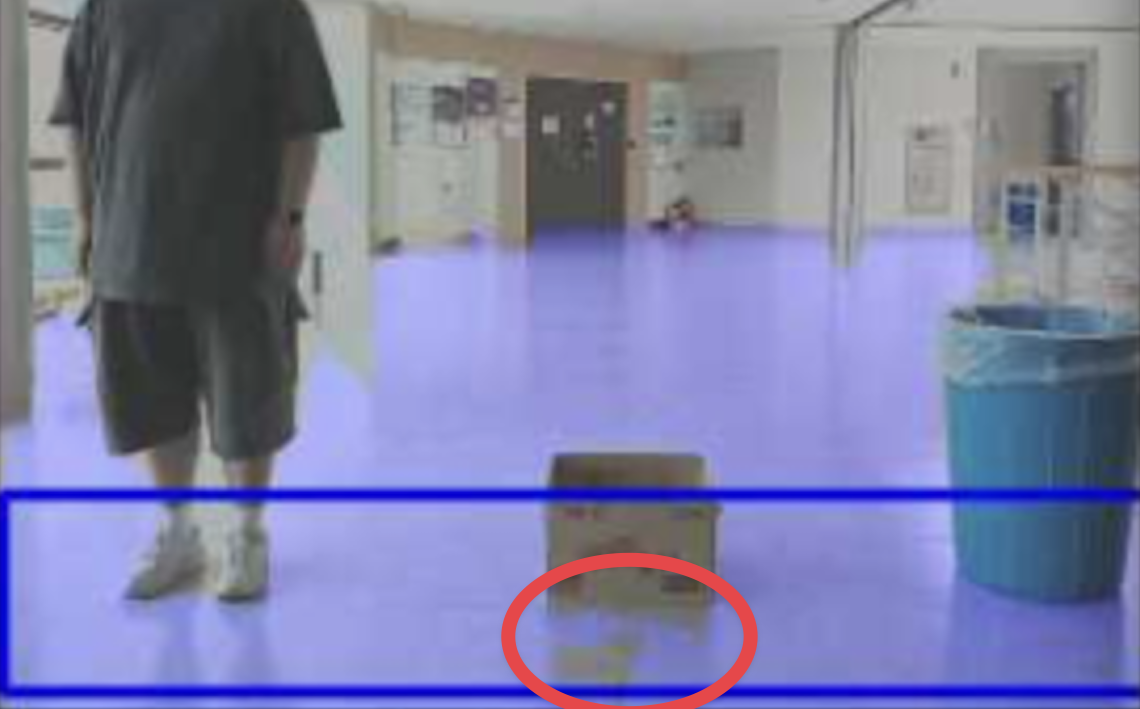
\includegraphics[width=0.88\linewidth]{segmentation_artifact}
  \caption{Example of segmentation noise under reflective ground surfaces. Specular glare can temporarily degrade boundary confidence, which our three-stage filtering pipeline mitigates.}
  \label{fig:seg_artifact}
\end{figure}

\begin{enumerate}
  \item \textbf{Obstacle Inflation Zone Overlap}: In both runs, the robot executed lateral evasion to $Y \approx +0.90\text{--}1.07$\,m. However, as the robot straightened out parallel to the obstacle ($X \approx 4.5$\,m, $Y \approx -0.4$\,m) and attempted to re-align with the nominal goal line ($Y=0$), the local path had to steer rightward. With configured Nav2 footprint radius $r_{\mathrm{footprint}} = 0.40$\,m (chassis radius $r_{\mathrm{robot}} = 0.33$\,m) and $r_{\mathrm{inflation}} = 0.90$\,m, the obstacle's total inflated cost radius was:
  \begin{equation}
    R_{\mathrm{zone}} = r_{\mathrm{footprint}} + r_{\mathrm{inflation}} = 0.40 + 0.90 = 1.30\,\text{m}.
  \end{equation}
  Measured from the obstacle boundary ($Y \approx -0.4$\,m), this high-cost zone extended up to $Y = +0.90$\,m, directly intersecting the robot's re-entry trajectory.
  \item \textbf{Local Planner Trajectory Rejection}: In the DWB controller, the obstacle avoidance critic weight was configured aggressively (\texttt{BaseObstacle.scale}\allowbreak\texttt{ = 8.0}). As the re-entry trajectory approached the obstacle's inflation boundary, all rightward candidate trajectories incurred prohibitive penalties. Simultaneously, straight and leftward trajectories incurred path distance penalties (\texttt{PathDist.scale}\allowbreak\texttt{ = 4.0}). Consequently, the DWB controller progressively decelerated the robot to a complete halt ($0.32 \rightarrow 0.18 \rightarrow 0.02 \rightarrow 0.00\,\text{m/s}$).
  \item \textbf{Recovery Server Simulation Clock Bug}: When forward progress stalled, Nav2 invoked its recovery behavior (\texttt{Wait}). However, a configuration mismatch in the recovery server (\texttt{use\_sim\_time: True} on the physical robot) caused the recovery action to wait indefinitely for a non-existent simulation clock (\texttt{/clock}), preventing automatic recovery.
\end{enumerate}
Remediating this behavior by reducing $r_{\mathrm{inflation}}$ to $0.55$\,m, lowering \texttt{BaseObstacle.scale} to $2.5$, and correcting \texttt{use\_sim\_time} ensures uninterrupted path re-alignment.

\subsection{Operational Boundaries in Confined Spaces and Geometric Scaling}
\label{subsec:corridor_limitations}
Conducting navigation trials in an open testing hall ($\sim 6$\,m wide) rather than confined corridors ($1.8\text{--}2.2$\,m) was essential due to camera geometry and costmap boundaries:

\begin{enumerate}
  \item \textbf{Lateral Proximity Blind Spot}: In a 2.0-meter corridor, a robot traveling along the centerline is only 1.0\,m away from both lateral walls. Because the minimum observable ground distance is $D_{\min} = 2.18$\,m (Section~\ref{sec:blind_spot}), ground contact points at angles $> 27^\circ$ fall entirely within the camera's blind spot. The robot cannot reliably perceive the lateral distance to adjacent walls.
  \item \textbf{Kinematic Swerve Clearance}: Evading a $0.4$\,m box produces an average lateral swerve of $Y = 1.22$\,m (Table~\ref{tab:exp2_results}). In a 2.0\,m corridor, even a minimal $0.50$\,m swerve places the robot footprint boundary ($0.50 + 0.40 = 0.90$\,m) within 10\,cm of the wall, whereas a $1.22$\,m swerve exceeds the 1.0\,m corridor half-width.
  \item \textbf{Inflation Trapping (Corridor Choke)}: When wall inflation costs ($1.30$\,m) project from both left and right walls, the lethal and inscribed cost zones overlap completely across the corridor width. Nav2's global and local planners view the entire corridor as an impassable obstacle, triggering immediate deadlocks.
\end{enumerate}
Consequently, conducting trials in a wide hall was essential to decouple pure obstacle perception from wall-induced costmap entrapment.

\subsection{Multi-Sensor Complementary Fusion Roadmap}
\label{subsec:sensor_fusion_roadmap}
While V-LiDAR facilitates obstacle avoidance without planar LiDAR in open, well-illuminated indoor environments, the $2.178$\,m optical blind spot remains a physical constraint of forward monocular vision. To deploy into narrow corridors ($<2.0$\,m), integrating two or three low-cost bumper ultrasonic transducers ($<\$5$) or miniature ToF sensors ($<\$8$, range $0.04\text{--}2.50$\,m) provides continuous proximity coverage in the $0.0\text{--}2.2$\,m zone. Ingesting sonar into a Nav2 \texttt{RangeSensorLayer} while V-LiDAR populates the primary long-range ($2.2\text{--}6.0$\,m) \texttt{ObstacleLayer} achieves full proximity coverage under \$40 total BOM.

\subsection{Dynamic Chassis Pitch Oscillations and IMU Compensation}
\label{subsec:dynamic_pitch}
The 2D Euclidean LUT (Section~\ref{subsec:lut}) assumes a static pitch angle ($\gamma = 2.0^\circ$). During aggressive acceleration or braking, suspension deflection induces transient pitch oscillations $\Delta \gamma \in [-1.5^\circ, +1.5^\circ]$. Differentiating~\eqref{eq:d_min} confirms that $\Delta \gamma = +1.0^\circ$ shifts estimated distance at 2.50\,m by $-0.097$\,m. To decouple robot dynamics from ranging precision on agile platforms, real-time pitch estimates $\hat{\gamma}_t = \gamma_0 + \Delta \gamma_{\mathrm{IMU}}$ from the onboard IMU can be fed into a parameterized distance formula:
\begin{equation}
  D_{\mathrm{dynamic}}(v, u) = \frac{h \cdot \sec(\theta(u))}{\tan(\phi(v) + \gamma_0 + \Delta \gamma_{\mathrm{IMU}})}.
  \label{eq:dynamic_pitch}
\end{equation}
In our 20 trials, the static LUT sufficed under cruising acceleration ($a \le 0.2\,\text{m/s}^2$, pitch deflection $<0.3^\circ$). Because trigonometric evaluation requires $<0.05\,\mu\text{s}$ per channel ($N_{\mathrm{ang}}=141$), \eqref{eq:dynamic_pitch} provides drop-in compensation without sacrificing real-time throughput.

\section{Conclusion and Future Work}
\label{sec:conclusion}

This paper presented V-LiDAR, an open-architecture monocular vision framework synthesizing ROS 2 \texttt{LaserScan} messages from YOLOv11n-seg floor masks as a low-cost perception alternative for mobile robot obstacle avoidance without physical LiDAR. Precomputed 2D Euclidean lookup tables eliminate runtime trigonometric projection, while multi-instance merging, $7 \times 7$ morphological closing, and asymmetric bidirectional persistence filtering suppress floor glare and transient flickers.

Theoretical formulation derived the near-field blind spot ($D_{\min} = 2.178$\,m for $h=1.05$\,m, $\gamma=2.0^\circ$), explaining costmap inflation entrapment in narrow corridors ($<2.2$\,m). OpenVINO FP16 acceleration achieves 78.4\,FPS (12.9\,ms latency) on an Intel Core Ultra 7 155H CPU, outperforming Depth Anything V2 Small (1.7\,FPS / 601.4\,ms) by up to $46.6\times$ and satisfying real-time 10\,Hz control deadlines. Across 20 real-world closed-loop trials without prior maps, the robot achieved a 90.0\% completion rate (18/20 runs) with 1.22\,m lateral clearance, while three-stage filtering suppressed reflection artifacts to 1.8\% and reduced jitter by 97.9\%. Future work will integrate bumper ultrasonic transducers for near-field coverage.

\section*{Acknowledgment}
This research was supported by the ANCHOR program Glocal University 30 through the Gyeongbuk ANCHOR CENTER, funded by the Ministry of Education (MOE) and the Gyeongsangbuk-do, Republic of Korea (2026-ANCHOR-15-119). This work was also supported in part by the National Research Foundation of Korea (NRF) grant funded by the Korean government (MSIT) (No. RS-2025-24683458) and the Handong Global University Academic Research Grant (No. 202500590001). Generative AI tools were utilized solely for English language editing and LaTeX formatting assistance; all research concepts, algorithmic designs, physical experimental validations, and manuscript conclusions were developed entirely by the authors.

\bibliographystyle{IEEEtran}
\bibliography{references}

\begin{IEEEbiography}[{
\includegraphics[width=1in,height=1.25in,clip,keepaspectratio]{hyunwoo.jpg}}]{Hyunwoo Gu}
was born in Seoul, South Korea, in 1999. He received the B.S. degree in computer science from Handong Global University, Pohang, South Korea, in 2025. He is currently pursuing the M.S. degree in the School of Computer Science and Electrical Engineering at Handong Global University. Since 2025, he has been with CGV Lab and a part-time research intern at the Korea Institute of Robot and Convergence (KIRO). His research interests include robotics, visual SLAM, artificial intelligence, and computer vision.
\end{IEEEbiography}

\begin{IEEEbiography}[{
\includegraphics[width=1in,height=1.25in,clip,keepaspectratio]{gunmin.jpg}}]{Gunmin Yoo}
was born in Seoul, South Korea, in 2000. He received the B.S. degree in computer science from Handong Global University, Pohang, South Korea, in 2025. He is currently pursuing the M.S. degree in the School of Computer Science and Electrical Engineering at Handong Global University. Since 2025, he has been with CGV Lab and a part-time research intern at the Korea Institute of Robot and Convergence (KIRO). His research interests include embodied artificial intelligence, vision-language navigation, and mobile robot perception.
\end{IEEEbiography}

\begin{IEEEbiography}[{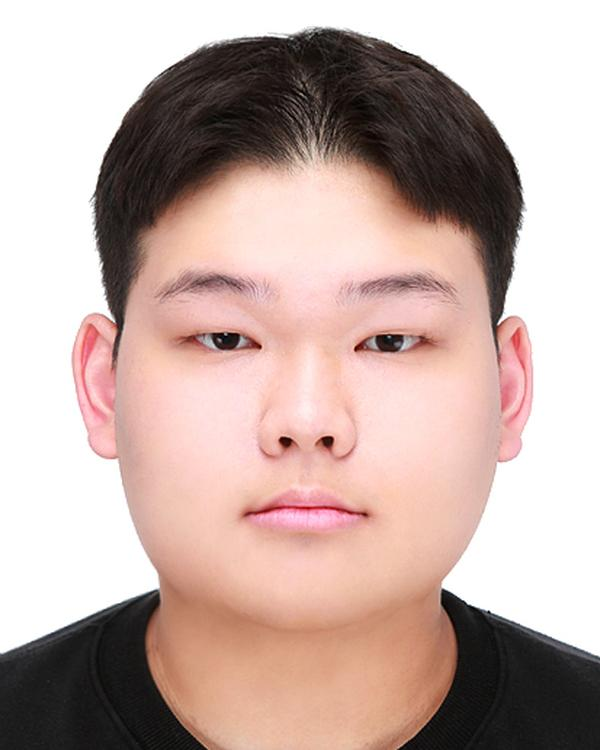
\includegraphics[width=1in,height=1.25in,clip,keepaspectratio]{hyunseo.jpg}}]{Hyunseo Lee}
was born in Busan, South Korea, in 2002. He is currently pursuing the B.S. degree in the School of Artificial Intelligence, Computer and Electrical Engineering at Handong Global University, Pohang, South Korea. Since 2025, he has been with the Computer Graphics and Vision Laboratory (CGV Lab) under the supervision of Prof. Sung Soo Hwang. His research interests include mobile robotics, vision-based perception, SLAM, and autonomous navigation.
\end{IEEEbiography}

\begin{IEEEbiography}[{
\includegraphics[width=1in,height=1.25in,clip,keepaspectratio]{hyunmo.png}}]{Hyun-Mo Kang}
is currently pursuing the B.S. degree in the School of Artificial Intelligence, Computer and Electrical Engineering at Handong Global University, Pohang, South Korea. Since 2025, he has been with the Computer Graphics and Vision Laboratory (CGV Lab) under the supervision of Prof. Sung Soo Hwang. His research interests include deep learning deployment, edge AI acceleration, autonomous robotics, and visual perception.
\end{IEEEbiography}

\begin{IEEEbiography}[{
\includegraphics[width=1in,height=1.25in,clip,keepaspectratio]{minseok.png}}]{Min-Seok Lee}
is currently pursuing the B.S. degree in the School of Artificial Intelligence, Computer and Electrical Engineering at Handong Global University, Pohang, South Korea. Since 2025, he has been with the Computer Graphics and Vision Laboratory (CGV Lab) under the supervision of Prof. Sung Soo Hwang. His research interests include mobile robotics, visual SLAM, robust navigation, and sensor fusion.
\end{IEEEbiography}

\begin{IEEEbiography}[{
\includegraphics[width=1in,height=1.25in,clip,keepaspectratio]{sungsoo.png}}]{Sung Soo Hwang}
was born in Busan, South Korea, in 1983. He received the B.S. degree in computer science and electrical engineering from Handong Global University, Pohang, South Korea, in 2008 and the M.S. and Ph.D. degrees in electrical engineering from the Korea Advanced Institute of Science and Technology (KAIST), Daejeon, South Korea, in 2010 and 2015, respectively. He is currently an Associate Professor with the School of Computer Science and Electrical Engineering, Handong Global University, Pohang, South Korea. His research interests include robotics, artificial intelligence, visual SLAM, and neural-rendering-based 3D reconstruction.
\end{IEEEbiography}

\EOD

\end{document}
